%%%%%%%%%%%%%%%%%%%%%%%%%%%%%%

%  Template LaTeX
%  classe: classe_PFC_IFBA_VDC.cls
%  compilador: pdfLaTeX ou XeLaTeX 
%
%  PFC - Projeto de Final de Curso Engenharia Elétrica (COEEL) - IFBA campus Vitória da Conquista e Modelo de Relatório
%
%  Este é um template (modelo) LaTeX que NÃO possui a intenção de seguir a norma ABNT-NBR14724 - Trabalhos Acadêmicos, porém estaremos seguindo as definições da norma ABNT-NBR6023 - Referências
%
%  Template criado para atender às demandas de Projeto Final de Curso (PFC) e Relatórios Técnicos de Engenharia Elétrica do IFBA campus Vitória da Conquista
%
%  versão 2023.08.07
%  Criado por: prof. Elvio Prado da Silva
%  elvio@ieee.org
%  https://github.com/prof-elvio
%
%  distribuição e modificação autorizada desde que mantenha os créditos das pessoas que trabalharam neste template
%%%%%%%%%%%%%%%%%%%%%%%%%%%%%%
\makeatletter % permitir que o símbolo @ seja usado em comandos de macro 
%%%%%%%%%%%%%%%%%%%%%%%%%%%%%%
%%%%%%%%%%%%%%%%%%%%%%%%%%%%%%
%%%%%% DOCUMENTCLASS %%%%%%%%%
%
% [pfc] caso seja PFC - Projeto Final de Curso
% [relatorio] caso seja RELATÓRIO de disciplina
% [preprojeto] caso seja Pré-Projeto de PFC
%
%
\documentclass[pfc]{./classe/cls-PFC-COEEL}
%\documentclass[relatorio]{./classe/cls-PFC-COEEL}
%\documentclass[preprojeto]{./classe/cls-PFC-COEEL}
%
%
%%%%%%%%%%%%%%%%%%%%%%%%%%%%%%
% ABNT-NBR6023 norma para citações bibliográficas
\usepackage[alf]{abntex2cite} 
%
% adicione aqui seus pacotes adicionais
% \usepackage{}
\usepackage{tikz}
\usetikzlibrary{positioning, arrows.meta, shapes.misc, fit}
%
%%%%%%%%%%%%%%%%%%%%%%%%%%%%
% Documento que cria a Capa e a folha de Rosto
%%%%%%%%%%%%%%%%%%%%%%%%%%%% 
% PREENCHA OS DADOS DA CAPA 
% DO SEU TRABALHO
%%%%%%%%%%%%%%%%%%%%%%%%%%%%
%%%% PREENCHER APENAS PARA PFC
%
\ifpfc
   \Titulo{Desenvolvimento de um Sistema Embarcado de Iluminação Adpatativa para Conformidade com a Norma ABNT NBR ISO/CIE 8995-1}
   \Autor{Enzo Carvalho Lisboa}
   \Orientador{\textbf{Orientador:} Diego Habib Santos Nolasco}
   \Coorientador{~}
   % se não houver coorientador
   % \Coorientador{~}
   % em PFCs é obrigatório que seja a data da defesa
   % \Data{23 de abril de 2023}    
   \Data{\today}   
   \Cidade{Vitória da Conquista-BA}
\fi 
%
%%%%%%%%%%%%%%%%%%%%%%%%%%%%
%%%% PREENCHER APENAS PARA RELATÓRIOS
% Relatórios: caso seja trabalho em grupo, 
% separe os nomes dos membros da equipe por \\
%
\ifrelatorio
   \Titulo{Modelo (Template) ~\LaTeX~ : Modelo de Relatório de Disciplinas - COEEL - IFBA {\it campus} Vitória da Conquista}
   \Autor{Nome do estudante 1 \\ Nome do estudante 2 \\ nome do estudante 3}
   \Professor{Nome do professor da disciplina}
   \Disciplina{Nome da Disciplina}
   \Data{\today}   
   \Cidade{Vitória da Conquista-BA}
\fi 
%
%%%%%%%%%%%%%%%%%%%%%%%%%%%%
%%%% PREENCHER APENAS PARA PRÉ PROJETOS
% Relatórios: caso seja trabalho em grupo, 
% separe os nomes dos membros da equipe por \\
%
\ifpreprojeto
   \Titulo{Desenvolvimento de um Sistema Embarcado de Iluminação Adpatativa para Conformidade com a Norma ABNT NBR ISO/CIE 8995-1}
   \Autor{Enzo Carvalho Lisboa}
   \Orientador{\textbf{Orientador:} Diego Habib Santos Nolasco}
   \Coorientador{~}
   % se não houver coorientador
   % \Coorientador{~}
   % em PFCs é obrigatório que seja a data da defesa
   % \Data{23 de abril de 2023}    
   \Data{\today}   
   \Cidade{Vitória da Conquista-BA}
\fi
%
%%%%%%%%%%%%%%%%%%%%%%%%%
%%%%%%%%%%%%%%%%%%%%%%%%%%%%
%%%%%%%%%%%%%%%%%%%%%%%%%%%%
%%%% CONFIGURA O ÍNDICE REMISSIVO
% configuração das letras em ./classe/estiloindice.ist
\makeindex[columns=3, title=ÍNDICE REMISSIVO, 
           options= -s ./classe/estiloindice.ist] 
%
%%%%%%%%%%%%%%%%%%%%%%%%%%%%
%%%% INICIA O PACOTE PARA GLOSSÁRIO
\loadglsentries{GLOSSARIO.tex}
% se é PFC 
\ifpfc 
    \makeglossaries
\fi 
% se é Pré-Projeto de PFC
\ifpreprojeto 
    \makeglossaries
\fi 
%
%
%%%%%%%%%%%%%%%%%%%%%%%%%%%% 
%%%%%%%%%%%%%%%%%%%%%%%%%%%%
%%%%% BEGIN DOCUMENT %%%%%%%
%%%%%%%%%%%%%%%%%%%%%%%%%%%%
%
%
\begin{document}

%%% 
%%%%%%%%%%%%%%%%%%%%%%%%%%%
% Este documento faz parte da classe cls-PFC-COEEL.cls
% NÃO ALTERE NENHUM DADO AQUI.
%%%%%%%%%%%%%%%%%%%%%%%%%%%
\pagestyle{EstiloPFC} % Estilo de página criado para o PFC do IFBA VDC
%%%% numeração da página em romano 
\pagenumbering{roman} 
%%%% espaçamento 1,5 entre linhas
\onehalfspacing
%%%%%%%%%%%%%%%%%%%%%%%%%%%%
%%%% CAPA 
%
% se é PFC faz capa de PFC

\ifpfc
    \CapaPFC
\fi 
    
% se é Relatório faz capa de Relatório
\ifrelatorio
    \CapaREL
\fi 

% se é Relatório faz capa de Pré-Projeto
\ifpreprojeto
    \CapaPREPROJETO
\fi 
%
%%%%%%%%%%%%%%%%%%%%%%%%%%%%
%%%% FOLHA DE ROSTO
% apenas para PFC
%
\ifpfc % se é PFC
    \newpage\clearpage\pagebreak
    \ifpdf\phantomsection\fi
    \addcontentsline{toc}{chapter}{Folha de Rosto}
    \FolhaRosto%
\fi 
\ifpreprojeto % se é Pré-Projeto
    \newpage\clearpage\pagebreak
    \ifpdf\phantomsection\fi
    \addcontentsline{toc}{chapter}{Folha de Rosto}
    \FolhaRosto%
\fi 
%
%%%%%%%%%%%%%%%%%%%%%%%%%%%%
%%%% FICHA CATALOGRÁFICA
% apenas para PFC
%
\ifpfc % se é PFC
    \newpage\clearpage\pagebreak
    \ifpdf\phantomsection\fi
    \addcontentsline{toc}{chapter}{Ficha Catalográfica}
    % inclua o PDF da ficha catalográfica feita pela biblioteca
    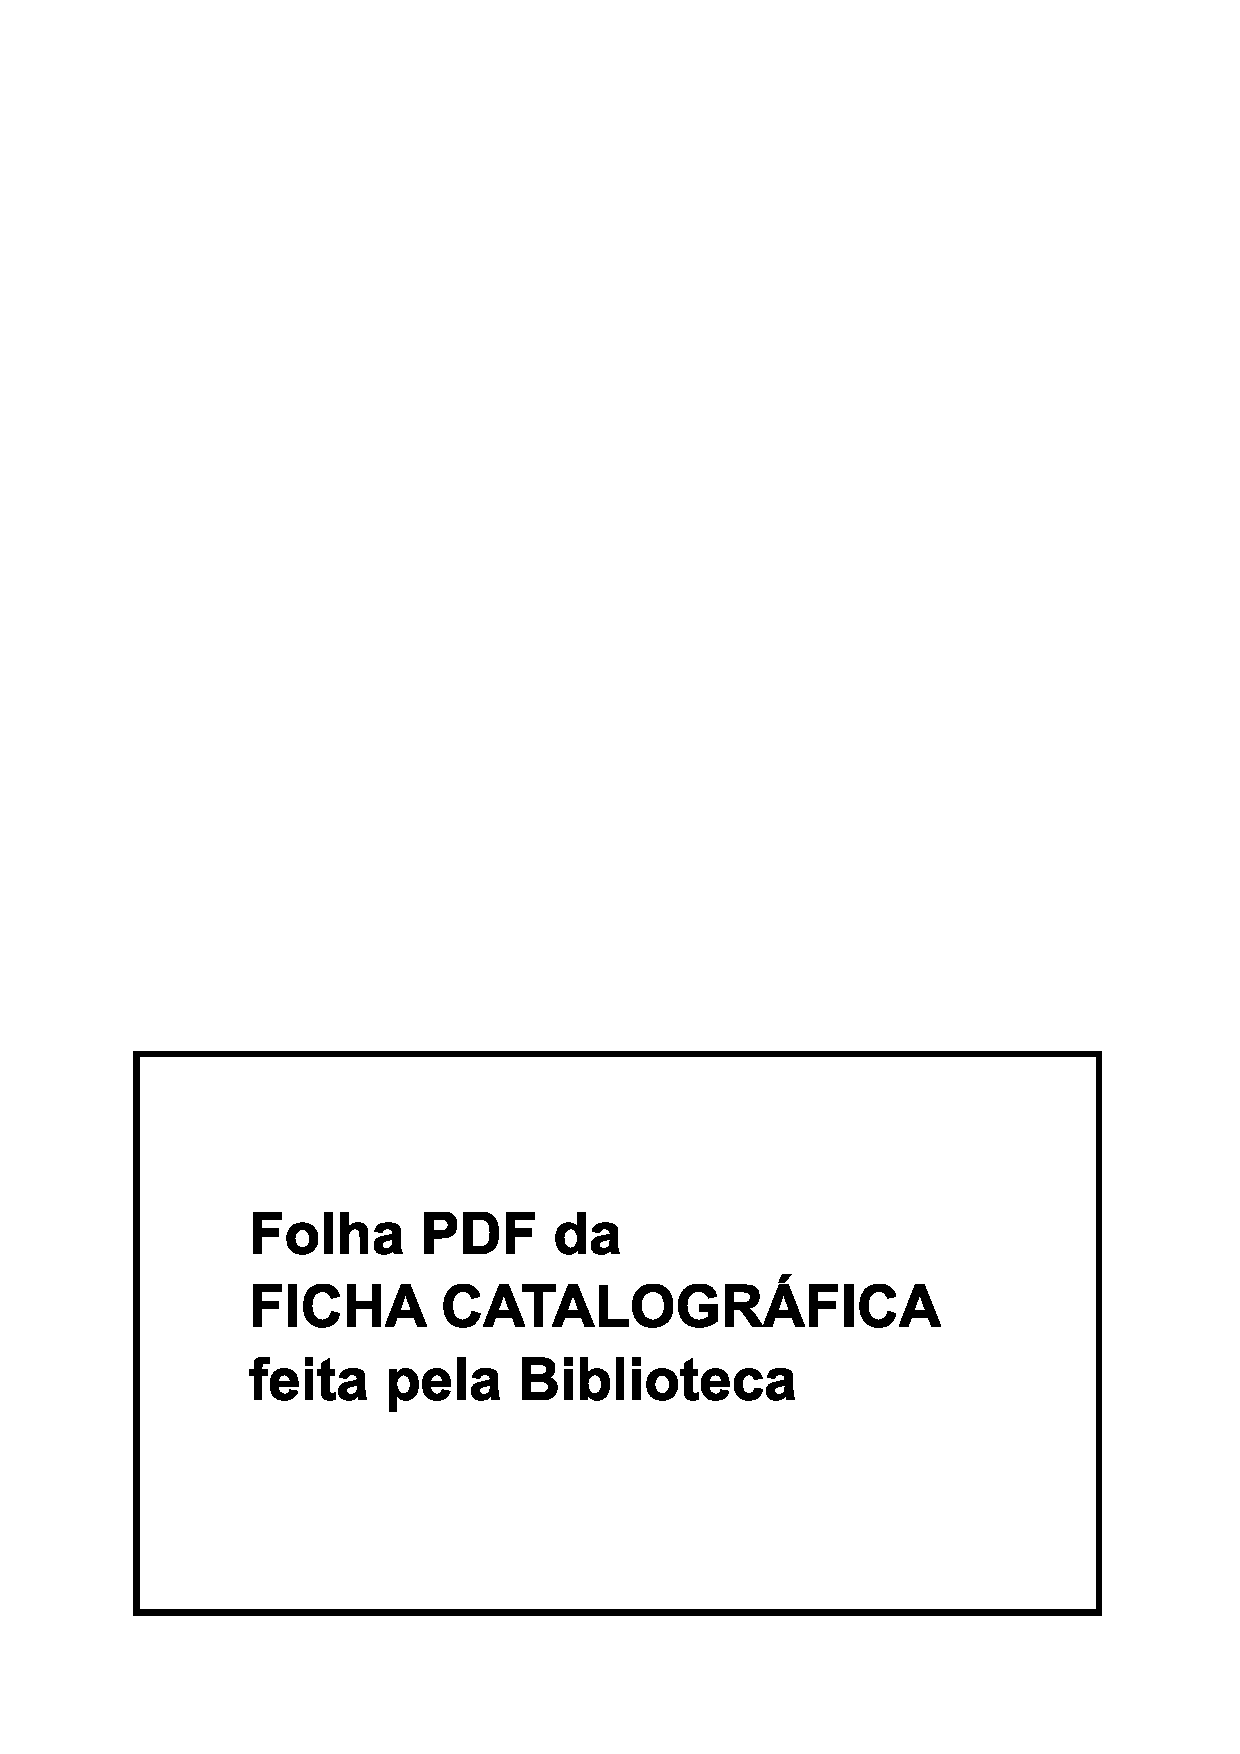
\includepdf[pages=1]{./PFC_Especificos/Ficha_Catalografica.pdf}
\fi 
%
%%%%%%%%%%%%%%%%%%%%%%%%%%%%
%%%% FOLHA DE APROVAÇÃO
% Apenas para PFC
%
\ifpfc % se é PFC
    \newpage\clearpage
    \ifpdf\phantomsection\fi
    \addcontentsline{toc}{chapter}{Folha de Aprovação}
    
    % inclua o PDF da folha de aprovação assinada digitalmente pelos membros da banca pelo SEI ou pelo SOU.GOV:

    % \includepdf[pages=1]{./PFC_Especificos/Folha_Aprovacao.pdf} % descomente esta linha quando for anexar o PDF

    % comente esta linha quando for anexar o PDF
    \include{./PFC_Especificos/b_FolhaAprovacao} 
\fi 
%
%%%%%%%%%%%%%%%%%%%%%%%%%%%
%%%% DEDICATÓRIA
% Apenas para PFC
%
\ifpfc % se é PFC
    \include{./PFC_Especificos/c_Dedicatoria}
\fi 
%
%%%%%%%%%%%%%%%%%%%%%%%%%%%%
%%%% AGRADECIMANTOS
% Apenas para PFC
%
\ifpfc % se é PFC
    \include{./PFC_Especificos/d_Agradecimentos}
\fi 
%
%%%%%%%%%%%%%%%%%%%%%%%%%%%%
%%%% RESUMO
% Apenas para PFC 
%
\ifpfc % se é PFC
    \newpage\clearpage
    \ifpdf\phantomsection\fi
    \addcontentsline{toc}{chapter}{Resumo}
    \include{./PFC_Especificos/e_Resumo}
\fi 
%
%%%%%%%%%%%%%%%%%%%%%%%%%%%%
%%%% ABSTRACT
% Apenas para PFC
%
\ifpfc % se é PFC
    \newpage\clearpage
    \ifpdf\phantomsection\fi
    \addcontentsline{toc}{chapter}{Abstract}
    \include{./PFC_Especificos/f_Abstract}
\fi 
%


%%%%%%%%%%%%%%%%%%%%%%%%%%%%
%%%% LISTA DE FIGURAS
% Apenas para PFC
%
\ifpfc % se é PFC
    \newpage\clearpage
    \ifpdf\phantomsection\fi
    \addcontentsline{toc}{chapter}{\listfigurename}
    \listoffigures
\fi 
%
%%%%%%%%%%%%%%%%%%%%%%%%%%%%
%%%% LISTA DE TABELAS
% Apenas para PFC
%
\ifpfc % se é PFC
    \clearpage\newpage
    \ifpdf\phantomsection\fi
    \addcontentsline{toc}{chapter}{\listtablename}
    \listoftables
\fi 
%
%%%%%%%%%%%%%%%%%%%%%%%%%%%%
%%%% LISTA DE CÓDIGOS
%
% Apenas para PFC
%
\ifpfc % se é PFC
    \clearpage\newpage
    \newcommand{\lstlistoflistingsname}{Lista de Códigos}
    \renewcommand{\lstlistingname}{Código}
    \addcontentsline{toc}{chapter}{Lista de Códigos\numberline{}}
    \lstlistoflistings
\fi 
%
%%%%%%%%%%%%%%%%%%%%%%%%%%%%
%%%% GLOSSÁRIO
%%%% LISTA DE SÍMBOLOS E SIGLAS
%
% https://pt.overleaf.com/learn/latex/Glossaries
%
% Glossário Apenas para PFC e Pré Projeto
%
\ifpfc % se é PFC
    \clearpage\newpage\pagebreak
    \renewcommand{\glossaryname}{Glossário: Símbolos e Siglas}
    \addcontentsline{toc}{chapter}{\glossaryname}
    \renewcommand{\pagelistname}{Páginas}%
    \printglossary[style=long3col-booktabs]
\fi
%
\ifpreprojeto % se é Pré Projeto de PFC
    \clearpage\newpage\pagebreak
    \renewcommand{\glossaryname}{Glossário: Símbolos e Siglas}
    \addcontentsline{toc}{chapter}{\glossaryname}
    \renewcommand{\pagelistname}{Páginas}%
    \printglossary[style=long3col-booktabs]
\fi
%
%%%%%%%%%%%%%%%%%%%%%%%%%%%%
%%%% SUMÁRIO
%
% Apenas para PFC e Pré-Projeto
%
\ifpfc % se é PFC
    \clearpage\pagebreak\newpage
    \renewcommand{\cftchapleader}{\cftdotfill{\cftdotsep}} % capítulos do sumário com linha de pontos
    \tableofcontents
\fi 
%
\ifpreprojeto  % se é Pré-Projeto
    \clearpage\pagebreak\newpage
    \renewcommand{\cftchapleader}{\cftdotfill{\cftdotsep}} % capítulos do sumário com linha de pontos
    \tableofcontents
\fi 
%
%%%%%%%%%%%%%%%%%%%%%%%%%%%%
%
\pagestyle{EstiloPFC} % estilo criado para este PFC
\clearpage\pagebreak\newpage
\onehalfspacing % espaçamento 1,5 entre linhas
\pagenumbering{arabic}  % numeração das páginas em algarismos arábicos
\makeatother %  restringir o uso do símbolo @ em comandos de macro
%
%%%%%%%%%%%%%%%%%%%%%%%%%%%%
%%%

% comentar esta linha para seu trabalho
%\include{Template} % utilizando o Template
%

%%%%%%%%%%%%%%%%%%%%%%%%%%%
\ifpfc % se é PFC
   % 
% Obrigatório em PFC e Pré-Projeto
% 
\chapter{Introdução}

%%%%%%%%%%%%%%%%%%%%%%%%%%%%%%%%%

A iluminação é um importante fator para garantir a segurança, o conforto e a eficiência em ambientes de trabalho. Uma iluminação adequada não apenas melhora a produtividade, mas também reduz riscos de acidentes e previne problemas de saúde, como fadiga ocular, dores de cabeça e transtornos posturais. Por outro lado, ambientes mal iluminados podem ser considerados insalubres, comprometendo a qualidade de vida dos trabalhadores e aumentando a probabilidade de erros e acidentes. Diante disso, normas técnicas como a Norma Brasileira (\gls{NBR}) 8995-1 da Associação Brasileira de Normas Técnicas (\gls{ABNT}) em conformidade com a Organização Internacional para Padronização (\gls{ISO}) e a Comissão Internacional de Iluminação (\gls{CIE}) e como a Norma de Higiene Ocupacional (\gls{NHO}) 11 estabelecem critérios mínimos de iluminância para diferentes tipos de ambientes e tarefas, visando promover um ambiente de trabalho seguro e produtivo.

A \gls{NBR} 8995-1 define os requisitos de iluminação para ambientes internos, estabelecendo níveis de iluminância, controle de ofuscamento e aspectos relacionados à qualidade da luz, como a reprodução de cores. Já a \gls{NHO} 11, desenvolvida pela Fundacentro, fornece diretrizes para a avaliação dos níveis de iluminância em ambientes de trabalho, incluindo procedimentos de medição e critérios de conformidade. Ambas as normas destacam a importância de uma iluminação adequada para a saúde e segurança dos trabalhadores, bem como para a eficiência energética.

No entanto, a manutenção dos níveis de iluminância recomendados pode ser um desafio, especialmente em ambientes dinâmicos onde as condições de iluminação natural variam ao longo do dia. Sistemas de iluminação convencionais, que operam com intensidade fixa, muitas vezes não são capazes de se adaptar a essas variações, resultando em desperdício de energia ou em níveis de iluminação inadequados. Nesse contexto, um sistema adpatativo de iluminação surge como uma solução promissora, permitindo o ajuste automático da intensidade luminosa com base nas condições do ambiente e nas necessidades específicas de cada tarefa.

A segurança do trabalho é diretamente impactada pela qualidade da iluminação. Ambientes mal iluminados dificultam a percepção de riscos, aumentando a probabilidade de acidentes. Além disso, a exposição prolongada a níveis inadequados de iluminação pode levar a problemas de saúde, como fadiga visual, estresse e até mesmo transtornos psicológicos. Por outro lado, uma iluminação bem planejada e ajustada às necessidades do ambiente pode melhorar a concentração, reduzir erros e aumentar a eficiência operacional.

A eficiência energética também é um aspecto crucial quando se fala em iluminação. Sistemas de iluminação adaptativa podem contribuir significativamente para a redução do consumo de energia, ajustando a intensidade luminosa conforme a necessidade real e aproveitando ao máximo a iluminação natural. Isso não apenas reduz os custos operacionais, mas também alinha-se às demandas contemporâneas de sustentabilidade e redução do impacto ambiental.

Os sistemas embarcados são dispositivos computacionais projetados para executar tarefas específicas, frequentemente em tempo real. Eles combinam hardware e software dedicados para garantir alto desempenho e eficiência energética. Esses sistemas estão presentes em diversos setores, incluindo automação industrial, dispositivos médicos, telecomunicações.

Este trabalho propõe o desenvolvimento de um sistema embarcado de iluminação adaptativa que se adapte dinamicamente às condições do ambiente, mantendo os níveis de iluminância em conformidade com as normas técnicas e de higiene ocupacional. O sistema utiliza sensores de luminosidade para monitorar a iluminação ambiente e um controlador Fuzzy para ajustar a intensidade luminosa de forma precisa e eficiente. Além disso, o sistema integra protocolos de comunicação sem fio e um cliente gráfico, permitindo a coleta e transmissão de dados em tempo real, bem como o controle remoto da iluminação.

A implementação de um sistema de iluminação adptativa não apenas garante o cumprimento das normas técnicas, mas também promove a eficiência energética, reduzindo o consumo de energia elétrica ao ajustar a iluminação conforme a necessidade real. Além disso, o sistema melhora a segurança e saúde dos trabalhadores, evitando problemas relacionados à má iluminação, como fadiga visual e acidentes de trabalho.

Com este trabalho, espera-se contribuir para a melhoria da qualidade da iluminação em ambientes de trabalho, promovendo a segurança, a saúde e a eficiência energética, alinhadas às demandas contemporâneas de sustentabilidade e conformidade com as normas técnicas.

%%%%%%%%%%%%%%%%%%%%%%%%%%%%%%%
% 
% Obrigatório em PFC e Pré-Projeto
% 
\section{Objetivo Geral}

Desenvolver um sistema de iluminação adaptativa que se adeque dinamicamente às condições do ambiente, mantendo os níveis de iluminância em conformidade com as normas técnicas \gls{NBR} 8995-1 e \gls{NHO} 11, visando promover a segurança, o conforto e a eficiência energética em ambientes de trabalho.
    
%%%%%%%%%%%%%%%%%%%%%%%%%%%%%%%
% 
% Obrigatório em PFC e Pré-Projeto
% 
\subsection{Objetivos Específicos}

\begin{enumerate}
    \item Realizar uma análise detalhada das normas \gls{NBR}  8995-1 e \gls{NHO} 11 para compreender os requisitos mínimos de iluminância e os critérios de avaliação em ambientes de trabalho;
    \item Projetar e implementar um sistema que utilize sensores de luminosidade, um controlador Fuzzy, um cliente \gls{PyQt5} e protocolos de comunicação como \gls{BLE} e \textit{WebSocket} para ajustar automaticamente a intensidade luminosa;
    \item Realizar testes para verificar a eficácia do sistema em manter os níveis de iluminância dentro dos limites recomendados pelas normas técnicas, comparando os resultados com medições de um luxímetro de referência;
    \item Demonstrar como o sistema de iluminação adaptativo pode reduzir o consumo de energia ao ajustar a iluminação conforme a necessidade real, contribuindo para a sustentabilidade;
    \item Elaborar um relatório técnico detalhado e apresentar os resultados obtidos, incentivando a aplicação do sistema em outros ambientes e futuras pesquisas na área de luminotécnica.
\end{enumerate}


%%%%%%%%%%%%%%%%%%%%%%%%%%%%%%%
% 
% Obrigatório em PFC e Pré-Projeto
% 

\section{Justificativa}

A iluminação inadequada no ambiente de trabalho pode causar uma série de problemas, como fadiga ocular, cansaço, dores de cabeça, estresse e até mesmo aumentar o risco de acidentes. Da mesma forma, um excesso de luz pode comprometer a segurança e o bem-estar, resultando em ofuscamento, desconforto visual e impactos negativos na saúde. Tanto a falta quanto o excesso de iluminação podem gerar erros nas atividades, comprometer a qualidade do trabalho e reduzir a produtividade \cite{ILO2007}. Pesquisas indicam que uma iluminação adequada proporciona benefícios significativos, incluindo maior eficiência e menos falhas. Há exemplos de fábricas onde ajustes na iluminação levaram a um aumento de 10\% na produtividade e uma redução de 30\% nos erros \cite{ILO1998}.

Em muitos ambientes industriais, a iluminação é composta por uma combinação de fontes naturais e artificiais. No entanto, nem sempre há um planejamento adequado que leve em consideração as necessidades específicas de cada tarefa. Muitas vezes, presume-se que todas as áreas da fábrica demandam o mesmo nível de iluminação, ignorando que diferentes tipos de trabalho exigem intensidades luminosas distintas para garantir conforto, precisão e eficiência. A melhoria na iluminação não significa necessariamente a necessidade de instalar mais fontes de luz ou aumentar o consumo de eletricidade. Em muitos casos, a solução está em otimizar o uso das luzes já disponíveis \cite{ILO2007}.

Além das questões de saúde e segurança ocupacional a eficiência energética é uma preocupação global. Segundo a Empresa de Pesquisa Energética (\gls{EPE}) no Brasil a demanda de energia elétrica irá triplicar até 2050. Mudanças nos comportamentos de consumo e em modelos de negócios, a eficiência energética e a eletrificação podem influenciar na necessidade de energia elétrica \cite{EPE2025}.

Em 2023, o consumo de energia per capita no Brasil ainda era metade do observado na União Europeia, indicando um potencial significativo para a adoção de práticas e tecnologias que promovam a eficiência energética \cite{EPE2025}. Quase 20\% do consumo de eletricidade em todo o mundo foi atribuído à eletricidade para iluminação \cite{UNEP2013}.

Nesse contexto, o desenvolvimento de um sistema de iluminação adaptativa, alinhados com normas como a ABNT NBR ISO/CIE 8995-1, torna-se essencial para garantir segurança laboral, o uso racional da energia e a conformidade com padrões internacionais.
 
   % 
% Obrigatório em PFC
% 

\chapter{Estado da Arte}

A história da iluminação é uma jornada que reflete a capacidade do homem em inovar e em se adaptar às necessidades de sua época. Durante primórdios da humanidade, o fogo era a única fonte de luz, utilizado para iluminação e socialização noturna. Há aproximadamente 1,5 milhões de anos, os ancestrais humanos aprenderam a conservar e utilizar o fogo, garantindo uma ferramenta essencial para o desenvolvimento social \cite{Guarnieri2015}.

Com o passar dos anos, novas formas de iluminação foram desenvolvidas. A iluminação dependia de combustíveis sólidos ou líquidos, como óleo de oliva, cera de abelha e óleo animal. No Egito Antigo, as lâmpadas eram feitas de cerâmica e abastecidas com óleos vegetais, sendo utilizadas em templos e residências. Na Roma Antiga, o uso de velas e tochas era comum, os romanos desenvolveram métodos para produção de velas, utilizando sebo animal e cera de abelha. Um caso excepcional foi registrado na china há cerca de 1700 anos, onde o gás natural era canalizado por tubos de bambu e utilizado como combustível \cite{James1995}. 

No século XVI, o óleo de baleia tornou-se um combustível lucrativo, especialmente após o início da caça às baleias no Atlântico Norte por nações europeias \cite{Proulx1968}. No entanto, foi apenas no final do século XVIII, com a Revolução Industrial, que o gás de carvão abriu caminho para uma tecnologia de iluminação mais avançada.

O primeiro sistema experimental de iluminação a gás foi intalado em 1784 pelo professor Jean-Pierre Minkelers na Universidade de Leuven, na Bélgica. A tecnologia foi aprimorada e levada ao Reino Unido por William Murdoch em 1792. Em 1807, Fredrick Winsor instalou uma rede de iluminação em Pall Mall, Londres que foi um sucesso comercial em áreas urbanas, em áreas rurais lâmpadas a óleo e velas ainda eram as únicas fontes de luz viávies \cite{Penzel1978}.

Em 1800, Alessandro Volta inventou a pilha elétrica, fornecendo uma fonte confiável de energia elétrica e permitindo experimentos científicos com iluminação elétrica. O químico inglês Humphry Davy demonstrou a primeira lâmpada elétrica em 1809, utilizando um grande conjunto de pilhas para gerar gerar uma descarga luminosa entre dois diodos de carvão, que apesar de uma intensa fonte de luz gerava muito calor e consumia muita energia, inviabilizando o uso doméstico \cite{Dredge2014}.

No final do século XIX os geradores elétricos começaram a se tornar mais eficientes, tornando a iluminação elétrica comercialmente viável. Entre as primeiras aplicações, destacam-se os experimentos do engenheiro russo Pawel Yablochkov, que desenvolveu a "vela de Yablochkov" uma lâmpada de arco de baixa potência \cite{Dredge2014}. 

A grande revolução ocorreu com a invenção da lâmpada incandescente. Joseph Swan e Thomas Edison foram pioneiros nessa tecnologia, e em 1879, Edison desenvolveu uma lâmpada de filamento de carbono que durava várias horas antes de se apagar. Isso permitiu a eletrificação em grande escala. Em 1882, Edison instalou a primeira rede elétrica comercial em Nova York, iluminando edifícios com lâmpadas incandescentes e inaugurando a era da eletricidade como principal fonte de luz \cite{Dredge2014}.

No início do século XX, a lâmpada incandescente passou por melhorias significativas. Em 1904, Sándor Just e Franjo Hanaman patentearam o filamento de tungstênio, que aumentou a eficiência das lâmpadas. Outra inovação importante foi a lâmpada de gás inerte, desenvolvida por Irwing Langmuir em 1913, que usava nitrogênio e argônio para prolongar a vida útil do filamento \cite{Bright1949}.

Além das lâmpadas incandescentes, novas tecnologias de iluminação surgiram, como a lâmpada de vapor de mercúrio, inventada por Peter Cooper Hewitt em 1901, a lâmpada de néon, criada por George Claude em 1909 e a lâmpada fluorescente em 1938 por Nikola Tesla \cite{Bright1949}.

O LED teve origem em 1907, quando Henry J. Round observou a emissão de luz em diodos de carbeto de silício, mas foi Oleg Losev, um cientista russo autodidata, quem realmente desenvolveu o conceito na década de 1920. Losev estudou a emissão de luz em diodos de carbeto de silício e zinco, compreendendo sua natureza não térmica. No entanto, suas contribuições foram esquecidas após sua morte em 1942. Na década de 1960, pesquisadores como Nick Holonyak redescobriram e consolidaram a tecnologia do LED \cite{Zheludev2007}. Desde os anos 2000, os LEDs se tornaram a principal opção de iluminação para residências, empresas e espaços públicos, promovendo sustentabilidade e economia de energia.


%%%%%%%%%%%%%%%%%%%%%%%%%%%%%

\chapter{Referencial Teórico}



\section{Sistemas Embarcados}

Os sistermas embarcados estão presentes em dispositivos do cotidiano, como eletrodomésticos e automóveis. Diferente dos computadores pessoais estes dispositivos são projetados para realizar tarefas específicas, combinando, software e periféricos de maneira dedicada \cite{Chase2007}. A demanda crescente por automação e eficiência energética impulsiona os estudos na área de sistemas embarcados, tornando-se essencial compreender seu desenvolvimento, funcionamento e aplicações. 

\subsection{Histórico e Evolução}

O conceito de sistemas embarcados surgiu no final da década de 1960, inicialmente aplicado ao controle de equipamentos telefônicos. Na época, os computadores eram grandes e caros, dificultando sua utilização em sistemas especializados \cite{Chase2007}.

Com o avanço da eletrônica e o desenvolvimento dos microprocessadores na década de 1970, tornou-se possível a criação de dispositivos menores e mais acessíveis. O desenvolvimento de linguagens de programação de mais alto nível também contribuiu para a popularização desses sistemas \cite{Chase2007}.

Nos dias atuais, os sistemas embarcados estão em constante evolução, incorporando inteligência artificial, aprendizado de máquina e conectividade com a internet, tornando-se elementos essenciais para a Indústria 4.0 \cite{Chase2007}.


\subsection{Conceitos e Características}

Um sistema é classificado como embarcado quando é dedicado a uma única tarefa e interage continuamente com o ambiente por meio de sensores e atuadores. A principal diferença entre um sistema embarcado e um sistema computacional genérico é que o primeiro tem sua arquitetura voltada para otimização e eficiência na execução de funções específicas \cite{Chase2007}.

As principais caracteríticas são:
\begin{itemize}
    \item \textbf{Capacidade computacional integrada:} São desenvolvidos para operar de maneira independente, sem a necessidade de interação constante do usuário.
    \item \textbf{Eficiência energética e autonomia:} Projetados para consumir pouca energia, muitas vezes operando com baterias de longa duração.
    \item \textbf{Interação com sensores e atuadores:} Captam informações do ambiente e tomam decisões em tempo real.
    \item \textbf{Software especializado:} Seu código é escrito de forma otimizada para um hardware específico.
    \item \textbf{Projeto voltado para aplicação específica:} Cada sistema embarcado é desenhado para atender a uma função específica, sem flexibilidade para outras tarefas.
\end{itemize}

%%%%%%%%%%%%%%%%%%%%%%%%%%%%%%%%%%%%%%%
\section{Controle}

O controle de sistemas variáveis é fundamental na engenharia, responsável por assegurar que sistemas físicos ou eletrônicos ajam conforme um comportamente escolhido. Geralmente o o controle objetiva ajustar variáveis como temperatura, velocidade ou iluminância, reduzindo o erro entre o valor medido e o valor de referência. Portanto a realimentação é o princípio bas edos sistemas de controle, permitindo a correção continua do desempenho do sistema, tornando-o mais preciso, estável e robusto diante das variações externas.

Em um modelo convencional de malha fechada, sensores medem a variável a ser controlada e o controlador processa a diferença entre os dados medidos e a referência, gerando um sinal de correção para os atuadores. O comportamento dinâmico é avaliado por critérios como tempo de acomodação, tempo de subida, sobressinal, erro em regime permanente e margem de estabilidade \cite{Franklin2013}.

Com os avanços da eletrônica e da computação, o controle migrou do domínio analógico, baseado em circuitos RC com amplificadores operacionais, para o digital, onde as variáveis são discretizadas e processadas digitalmente. Essa mudança introduziu o uso da trasnformada Z como ferramenta matemática para representar e analisar sistemas de controle.

Em sistemas de controle digital os sinais analógicos medidos pelos sensores são convertidos em valores numéricos por conversores A/D. Esses valores são processados por algorítimos no microcontrolador, resultando em um sinal de saída digital que é transformado por conversores D/A em um sinal analógico que vai acionar os atuadores. \cite{Ogata2010}.

\subsection{Lógica Fuzzy}
A lógica fuzzy é uma extensão da lógica clássica que permite representar incertezas e variações contínuas. Diferente da lógica booleana, que trabalha apenas com valores verdadeiros ou falsos, a lógica fuzzy utiliza graus de pertinência entre 0 e 1, permitindo que uma variável pertença parcialmente a diferentes conjuntos.

Nos sistemas de controle, essa abordagem é útil quando o modelo matemático da planta é difícil de determinar. Em vez de equações exatas, o comportamento é definido por regras linguísticas, que descrevem como o sistema deve reagir a cada situação, de forma semelhante ao raciocínio humano \cite{Habib-Doutorado}.

Um controlador fuzzy é composto por três etapas principais:
\begin{itemize}
    \item Fuzzificação, que converte as variáveis de entrada em valores linguísticos usando funções de pertinência;
    \item Inferência, onde as regras “SE... ENTÃO...” são aplicadas para determinar as respostas possíveis;
    \item Defuzzyficação, que transforma o resultado difuso em um valor numérico de saída.
\end{itemize}

Assim, a lógica fuzzy possibilita um controle adaptativo e eficiente, capaz de atuar mesmo sob incertezas e mudanças nas condições do ambiente. Essa característica faz com que o controlador fuzzy seja adequado para aplicações de iluminação inteligente, combinando simplicidade de implementação com desempenho robusto.


\subsection{Controle por Corte de Fase}
O controle por corte de fase é muito utilizado para controle de potência a cargas em sistemas \gls{CA}. Diferente da Modulação por Largura de Pulso (\gls{PWM}), que varia o tempo de condução em um ciclo de trabalho fixo, o corte de fase controla o momento em que a tensão \gls{CA} é aplicada a carga, cortando uma parte da onda senoidal em cada ciclo. Esssa técnica é eficaz para cargas resistivas ou indutivas, como lâmpadas e motores \gls{CA}

\subsubsection{Funcionamento}

Essa técnica funciona interrompendo parte da onda senoidal da tensão \gls{CA} em cada semiciclo. O ângulo de disparo determina o ponto no qual o \gls{TRIAC} é acionado, permitindo que a corrente flua para a carga. Quanto maior o ângulo de disparo, menor será a potência entregue à carga \cite{Rashid2014}.

A relação entre o ângulo de disparo e a potência pode ser expressa pela Equação \ref{eq:potencia_corte_fase}.

\begin{equation}
     P = P_{\text{max}} \left(1 - \frac{\alpha}{\pi} + \frac{\sin(2\alpha)}{2\pi}\right)
    \label{eq:potencia_corte_fase}
\end{equation}

Sendo que:\\
\vspace{-1.5cm}
\begin{tabbing}
    \hspace{1cm}  \= \hspace{1cm} \= \kill \\
    \gls{P}       \> \(\Rightarrow\) \> Potência média entregue à carga; \\
    \gls{Pmax} \> \(\Rightarrow\) \> Potência máxima (quando \(\alpha = 0\)); \\
    \gls{alpha}    \> \(\Rightarrow\) \> Ângulo de disparo em radianos; \\
    \gls{pi}     \> \(\Rightarrow\) \> Constante pi (\(\approx 3.1416\)); \\
\end{tabbing}



%%%%%%%%%%%%%%%%%%%%%%%%%%%%%%%%%%%%%%%
\section{Normas Técnicas}

\subsection{ABNT NBR ISO/CIE 8995-1}

A \gls{NBR} 8995-1 \cite{ISOCIE} estabelece os requisitos para a iluminação de ambientes de trabalho internos, visando garantir que as tarefas visuais sejam realizadas de forma eficiente, segura e confortável. A norma abrange tanto aspectos quantitativos, como os níveis de iluminância, quanto aspectos qualitativos, como a distribuição da luminância, o controle do ofuscamento e a reprodução de cores. O objetivo principal é proporcionar um ambiente luminoso que promova o bem-estar, a segurança e a produtividade dos trabalhadores.

A norma é aplicável a uma ampla variedade de ambientes de trabalho, desde escritórios até instalações industriais, e considera tanto a iluminação artificial quanto a natural. Além disso, a \gls{NBR} 8995-1 fornece diretrizes para o planejamento, projeto e verificação de sistemas de iluminação, garantindo que os requisitos mínimos sejam atendidos.

\subsubsection{Critérios de Projeto de Iluminação}
\paragraph{Ambiente Luminoso}

O ambiente luminoso é um fator crucial para o desempenho visual e o conforto dos trabalhadores. A norma define que uma boa iluminação deve proporcionar:

\begin{itemize}
    \item \textbf{Conforto visual:} Sensação de bem-estar e conforto para os trabalhadores.
    \item \textbf{Desempenho visual:} Capacidade de realizar tarefas visuais de forma rápida e precisa, mesmo em condições desafiadoras.
    \item \textbf{Segurança visual:} Detecção de perigos e movimentação segura no ambiente de trabalho.
\end{itemize}

\paragraph{Distribuição da Luminância}

A distribuição da luminância no campo de visão é essencial para a adaptação dos olhos e a visibilidade das tarefas. A norma recomenda que a luminância seja bem balanceada, evitando contrastes excessivos que possam causar fadiga visual ou desconforto. A luminância das superfícies internas, como teto, paredes, planos de trabalho e piso, deve ser cuidadosamente considerada, com faixas de refletância recomendadas para cada superfície.


Para alcançar esses objetivos, a norma estabelece parâmetros como a distribuição da luminância, a iluminância, o controle do ofuscamento, a direcionalidade da luz, a aparência e a reprodução de cores, a cintilação, a luz natural e a manutenção do sistema de iluminação.

\paragraph{Iluminância}

A iluminância é a quantidade de luz que incide sobre uma superfície e é medida em lux (\gls{lux}). A norma estabelece valores mínimos de iluminância mantida para diferentes tipos de tarefas e ambientes. A iluminância mantida é o valor abaixo do qual a iluminância média não deve cair durante o período de uso do sistema de iluminação.

A norma também define uma escala de iluminância, que varia de 20 \gls{lux} a 5000 \gls{lux}, dependendo da complexidade da tarefa visual. Para tarefas que exigem maior precisão, como trabalhos de inspeção ou leitura de documentos, são recomendados níveis mais altos de iluminância. Além disso, a iluminância no entorno imediato da área de tarefa deve ser proporcional à iluminância da tarefa, garantindo uma distribuição uniforme da luz.

\paragraph{Ofuscamento}
O ofuscamento é uma sensação visual desagradável causada por fontes de luz excessivamente brilhantes ou por reflexões em superfícies especulares. A norma classifica o ofuscamento em duas categorias:

\begin{itemize}
    \item \textbf{Ofuscamento desconfortável:} Causa desconforto visual, mas não impede a realização da tarefa.
    \item \textbf{Ofuscamento incapacitante:} Prejudica diretamente a visão, podendo levar a erros ou acidentes.
\end{itemize}

Para controlar o ofuscamento, a norma recomenda o uso de luminárias com ângulos de corte adequados e a limitação da luminância das superfícies brilhantes. O Índice de Ofuscamento Unificado (\gls{UGR}) é utilizado para quantificar o nível de desconforto causado pelo ofuscamento, com valores máximos recomendados para diferentes tipos de ambientes.

\paragraph{Direcionalidade da Luz}

A direcionalidade da luz influencia a modelagem do ambiente e a visibilidade das tarefas. A norma recomenda que a luz seja direcionada de forma a destacar objetos e revelar texturas, sem criar sombras excessivas. A iluminação direcional é particularmente importante para tarefas que envolvem detalhes finos, como trabalhos de gravação ou inspeção.

\paragraph{Aspectos da Cor}

A aparência e a reprodução de cores são fatores importantes para o conforto visual e a precisão das tarefas. A norma define três categorias de temperatura de cor correlata (\gls{Tcp}):

\begin{itemize}
    \item \textbf{Luz quente:} Abaixo de 3300 Kelvin (\gls{kelvin}).
    \item \textbf{Luz intermediária:} Entre 3300 \gls{kelvin} e 5300 \gls{kelvin}.
    \item \textbf{Luz fria:} Acima de 5300 \gls{kelvin}. 
\end{itemize}

A escolha da temperatura de cor depende do ambiente e da tarefa, sendo que a luz fria é geralmente preferida em climas quentes, enquanto a luz quente é mais adequada para climas frios. Além disso, a norma estabelece valores mínimos para o índice geral de reprodução de cor (\gls{Ra}), que mede a capacidade da fonte de luz de reproduzir cores de forma fiel. Para a maioria dos ambientes de trabalho, o \gls{Ra} mínimo recomendado é 80.

\paragraph{Luz Natural}

A luz natural é uma fonte importante de iluminação e pode ser utilizada para complementar ou substituir a iluminação artificial. A norma recomenda que a luz natural seja controlada para evitar ofuscamento e desconforto térmico, especialmente em áreas próximas a janelas. Além disso, a norma sugere o uso de sistemas de dimerização ou controle automático para integrar a luz natural e artificial de forma eficiente.

\paragraph{Manutenção do Sistema de Iluminação}

A manutenção do sistema de iluminação é essencial para garantir que os níveis de iluminância sejam mantidos ao longo do tempo. A norma recomenda que o projeto de iluminação inclua um plano de manutenção, com a substituição periódica das lâmpadas e a limpeza das luminárias e superfícies do ambiente. O fator de manutenção, que considera a depreciação do fluxo luminoso das lâmpadas e o acúmulo de sujeira, deve ser calculado para garantir que a iluminância mantida seja alcançada.

\subsubsection{Requisitos para o Planejamento da Iluminação}

A norma ISO/CIE 8995-1 fornece diretrizes detalhadas para o planejamento da iluminação em diferentes tipos de ambientes e atividades. A norma apresenta os requisitos de iluminância, Índice de Ofuscamento Unificado Limite \gls{UGRL} e do \gls{Ra} para uma variedade de ambientes, como escritórios, escolas, hospitais, indústrias e áreas de varejo.

Por exemplo, para um escritório onde são realizadas tarefas de leitura e escrita, a norma recomenda uma iluminância mantida de 500 \gls{lux}, um \gls{UGRL} máximo de 19 e um \gls{Ra} mínimo de 80. Já para uma sala de cirurgia, a iluminância recomendada é de 1000 \gls{lux}, com um \gls{UGRL} máximo de 19 e um \gls{Ra} mínimo de 90.

\subsubsection{Procedimentos de Verificação}

A norma também estabelece procedimentos para a verificação do sistema de iluminação, garantindo que os requisitos sejam atendidos. Isso inclui a medição da iluminância em pontos específicos, a verificação do \gls{UGR} e a avaliação do \gls{Ra}. Além disso, a norma recomenda a documentação do fator de manutenção e a realização de medições periódicas para garantir que o sistema de iluminação continue a atender aos requisitos ao longo do tempo.

\subsubsection{Considerações sobre Energia}

A eficiência energética é um aspecto importante do projeto de iluminação. A norma recomenda que o sistema de iluminação seja projetado para atender aos requisitos de iluminação sem desperdício de energia. Isso pode ser alcançado através da seleção de equipamentos eficientes, como lâmpadas de baixo consumo e sistemas de controle automático, que ajustam a iluminação de acordo com a disponibilidade de luz natural e a ocupação do ambiente.

%%%%%%%%%%%%%%%%%%%%%%%%%%%%%

\subsection{NHO 11}

A \gls{NHO} 11 \cite{NHO11}, intitulada "Avaliação dos níveis de iluminamento em ambientes internos de trabalho", estabelece critérios e procedimentos técnicos para a avaliação dos níveis de iluminância em ambientes de trabalho internos. A norma foi desenvolvida pela Fundacentro (Fundação Jorge Duprat Figueiredo de Segurança e Medicina do Trabalho) e substituiu a antiga NHT 10-I/E de 1986, trazendo atualizações importantes em relação às práticas de medição e avaliação da iluminação.

A norma é uma ferramenta essencial para garantir que os ambientes de trabalho atendam aos requisitos mínimos de iluminância, promovendo a segurança, o conforto e a eficiência dos trabalhadores. A norma aborda tanto aspectos quantitativos, como a medição da iluminância, quanto aspectos qualitativos, como a avaliação de ofuscamento, cintilação e distribuição da luz.

\subsubsection{Objetivos e Aplicação}

O principal objetivo da \gls{NHO} 11 é estabelecer critérios e procedimentos para a avaliação dos níveis de iluminância em ambientes internos de trabalho, indicando os principais parâmetros que interferem na qualidade da iluminação. A norma se aplica a qualquer ambiente de trabalho interno, independentemente do setor ou atividade, e pode ser utilizada por profissionais de segurança do trabalho, engenheiros, arquitetos e técnicos responsáveis pela avaliação e manutenção dos sistemas de iluminação.

A norma também aborda a detecção de não conformidades que possam comprometer a segurança e o desempenho dos trabalhadores, como ofuscamento, cintilação e efeitos estroboscópicos.

\subsubsection{Procedimentos de Avaliação}

A \gls{NHO} 11 estabelece um procedimento detalhado para a avaliação dos níveis de iluminância, que inclui:

\begin{itemize}
    \item \textbf{Avaliação Preliminar:} Antes de realizar as medições, é necessário fazer uma avaliação preliminar do ambiente de trabalho. Essa avaliação inclui a verificação de aspectos como ofuscamento, cintilação, efeito estroboscópico, direcionalidade da luz, sombras excessivas, aparência da cor e contraste. A norma fornece uma lista de verificação, que auxilia na identificação de problemas e na proposição de melhorias.
    \item \textbf{Abordagem dos Locais e Condições de Trabalho:} É necessário identificar as atividades realizadas no ambiente, as áreas de tarefa e as áreas de trabalho. A descrição do ambiente de trabalho, incluindo o sistema de iluminação utilizado, tipos de luminárias e lâmpadas, é fundamental para a realização das medições. A norma recomenda que as medições sejam realizadas sob as condições mais desfavoráveis, como em dias nublados, para garantir que os resultados dependam apenas da iluminação artificial.
    \item \textbf{Equipamentos de Medição:} Os medidores de iluminância (luxímetros) devem ser calibrados e certificados pelo Inmetro (Instituto Nacional de Metrologia, Qualidade e Tecnologia) ou por laboratórios acreditados. O equipamento deve ser capaz de medir a iluminância em diferentes tipos de lâmpadas, como LED, fluorescente e vapor de sódio. A calibração deve ser realizada periodicamente, conforme as recomendações do fabricante ou sempre que houver suspeita de dano no equipamento.
    \item \textbf{Procedimento de Medição:} As medições devem ser realizadas com o sistema de iluminação em operação normal. A leitura deve ser feita no plano da tarefa visual, que pode ser horizontal, vertical ou inclinado. Quando o plano da tarefa não for definido, a medição deve ser realizada a 0,75 m do piso. A norma detalha os procedimentos para a determinação da iluminância média em ambientes retangulares, considerando diferentes configurações de luminárias.
\end{itemize}

\subsubsection{Critérios de Avaliação}

A \gls{NHO} 11 estabelece que a avaliação do nível de iluminância deve ser feita ponto a ponto, comparando os valores medidos com os níveis mínimos de iluminância recomendados para cada tipo de tarefa ou atividade. A norma permite uma tolerância de 10\% abaixo do valor mínimo recomendado. Além disso, a iluminância medida na área da tarefa não deve ser inferior a 70\% da iluminância média do ambiente.

A norma também define critérios para a uniformidade da iluminância, recomendando que a razão entre o maior valor de iluminância medido na área da tarefa e a iluminância média do ambiente não seja superior a 5:1. Para áreas de trabalho adjacentes, a razão da iluminância média não deve ultrapassar 5:1.

\subsubsection{Manutenção do Sistema de Iluminação}

A \gls{NHO} 11 enfatiza a importância da manutenção preventiva e corretiva do sistema de iluminação. A limpeza das luminárias, a substituição de lâmpadas e a verificação periódica dos níveis de iluminância são essenciais para garantir que o sistema de iluminação continue a atender aos requisitos mínimos. A periodicidade da manutenção depende das características do ambiente de trabalho, como a sujidade e o tipo de atividade realizada.

\subsubsection{Relatório de Avaliação}

A norma estabelece que o relatório técnico deve documentar todos os aspectos da avaliação, incluindo:

\begin{itemize}
    \item Introdução, com os objetivos do trabalho e justificativa;
    \item Instrumental utilizado e certificado de calibração;
    \item Critérios e procedimentos de avaliação adotados;
    \item Descrição do ambiente de trabalho, atividades realizadas e sistema de iluminação;
    \item Dados obtidos, incluindo parâmetros quantitativos e qualitativos;
    \item Interpretação dos resultados e recomendações.
\end{itemize}

O relatório deve ser claro e detalhado, permitindo que os responsáveis pela manutenção do sistema de iluminação possam tomar as medidas necessárias para corrigir eventuais não conformidades.



%%%%%%%%%%%%%%%%%%%%%%%%%%%%%
   % 
% Obrigatório em PFC
%
\chapter{Metodologia}

O presente projeto foi desenvolvido por meio de uma abordagem \textbf{aplicada, experimental e quantitativa}, com foco na implementação de um \textbf{sistema embarcado de iluminação adaptativa} em conformidade com as normas \gls{NBR} 8995-1 e \gls{NHO} 11. O método adotado envolveu o desenvolvimento do sistema embarcado, seguido por testes experimentais e validação dos resultados obtidos. As etapas metodológicas foram organizadas da seguinte forma:

\begin{itemize}
    \item \textbf{Desenvolvimento do Sistema Embarcado} – O sistema foi dividido em três módulos principais: sensores, controlador e supervisório.
    \begin{itemize}
        \item \textbf{Sensores} – Responsáveis pelas leituras periódicas de iluminância e transmissão dos dados ao controlador. Foram implementados modos de economia de energia para reduzir o consumo durante períodos de inatividade.

        \item \textbf{Controlador} – Executa o algoritmo de controle fuzzy, ajustando a potência luminosa por meio de um circuito de corte de fase com detecção de cruzamento por zero e acionamento por TRIAC.

        \item \textbf{Supervisório} – Desenvolvido em \textit{Python}, permite o monitoramento em tempo real, com registro automático em arquivos e geração de gráficos.
    \end{itemize}

    \item \textbf{Testes Experimentais} – O sistema foi instalado em ambiente real e submetido a diferentes condições de iluminação natural e artificial. Durante os testes, foram registrados valores de iluminância, potência da lâmpada e comportamento do controle fuzzy.

    \item \textbf{Validação dos Resultados} – Com base nos dados obtidos, foi avaliada a capacidade do sistema em manter os níveis de iluminância próximos ao setpoint definido, bem como a eficiência energética alcançada.
\end{itemize}

Todas as etapas foram integradas em ambiente controlado, com o sistema operando em tempo real, o que permitiu validar a eficiência do controle fuzzy no ajuste automático da intensidade luminosa.




\fi 
\ifpreprojeto % se é Pré-Projeto
   % 
% Obrigatório em PFC e Pré-Projeto
% 
\chapter{Introdução}

%%%%%%%%%%%%%%%%%%%%%%%%%%%%%%%%%

A iluminação é um importante fator para garantir a segurança, o conforto e a eficiência em ambientes de trabalho. Uma iluminação adequada não apenas melhora a produtividade, mas também reduz riscos de acidentes e previne problemas de saúde, como fadiga ocular, dores de cabeça e transtornos posturais. Por outro lado, ambientes mal iluminados podem ser considerados insalubres, comprometendo a qualidade de vida dos trabalhadores e aumentando a probabilidade de erros e acidentes. Diante disso, normas técnicas como a Norma Brasileira (\gls{NBR}) 8995-1 da Associação Brasileira de Normas Técnicas (\gls{ABNT}) em conformidade com a Organização Internacional para Padronização (\gls{ISO}) e a Comissão Internacional de Iluminação (\gls{CIE}) e como a Norma de Higiene Ocupacional (\gls{NHO}) 11 estabelecem critérios mínimos de iluminância para diferentes tipos de ambientes e tarefas, visando promover um ambiente de trabalho seguro e produtivo.

A \gls{NBR} 8995-1 define os requisitos de iluminação para ambientes internos, estabelecendo níveis de iluminância, controle de ofuscamento e aspectos relacionados à qualidade da luz, como a reprodução de cores. Já a \gls{NHO} 11, desenvolvida pela Fundacentro, fornece diretrizes para a avaliação dos níveis de iluminância em ambientes de trabalho, incluindo procedimentos de medição e critérios de conformidade. Ambas as normas destacam a importância de uma iluminação adequada para a saúde e segurança dos trabalhadores, bem como para a eficiência energética.

No entanto, a manutenção dos níveis de iluminância recomendados pode ser um desafio, especialmente em ambientes dinâmicos onde as condições de iluminação natural variam ao longo do dia. Sistemas de iluminação convencionais, que operam com intensidade fixa, muitas vezes não são capazes de se adaptar a essas variações, resultando em desperdício de energia ou em níveis de iluminação inadequados. Nesse contexto, um sistema adpatativo de iluminação surge como uma solução promissora, permitindo o ajuste automático da intensidade luminosa com base nas condições do ambiente e nas necessidades específicas de cada tarefa.

A segurança do trabalho é diretamente impactada pela qualidade da iluminação. Ambientes mal iluminados dificultam a percepção de riscos, aumentando a probabilidade de acidentes. Além disso, a exposição prolongada a níveis inadequados de iluminação pode levar a problemas de saúde, como fadiga visual, estresse e até mesmo transtornos psicológicos. Por outro lado, uma iluminação bem planejada e ajustada às necessidades do ambiente pode melhorar a concentração, reduzir erros e aumentar a eficiência operacional.

A eficiência energética também é um aspecto crucial quando se fala em iluminação. Sistemas de iluminação adaptativa podem contribuir significativamente para a redução do consumo de energia, ajustando a intensidade luminosa conforme a necessidade real e aproveitando ao máximo a iluminação natural. Isso não apenas reduz os custos operacionais, mas também alinha-se às demandas contemporâneas de sustentabilidade e redução do impacto ambiental.

Os sistemas embarcados são dispositivos computacionais projetados para executar tarefas específicas, frequentemente em tempo real. Eles combinam hardware e software dedicados para garantir alto desempenho e eficiência energética. Esses sistemas estão presentes em diversos setores, incluindo automação industrial, dispositivos médicos, telecomunicações.

Este trabalho propõe o desenvolvimento de um sistema embarcado de iluminação adaptativa que se adapte dinamicamente às condições do ambiente, mantendo os níveis de iluminância em conformidade com as normas técnicas e de higiene ocupacional. O sistema utiliza sensores de luminosidade para monitorar a iluminação ambiente e um controlador Fuzzy para ajustar a intensidade luminosa de forma precisa e eficiente. Além disso, o sistema integra protocolos de comunicação sem fio e um cliente gráfico, permitindo a coleta e transmissão de dados em tempo real, bem como o controle remoto da iluminação.

A implementação de um sistema de iluminação adptativa não apenas garante o cumprimento das normas técnicas, mas também promove a eficiência energética, reduzindo o consumo de energia elétrica ao ajustar a iluminação conforme a necessidade real. Além disso, o sistema melhora a segurança e saúde dos trabalhadores, evitando problemas relacionados à má iluminação, como fadiga visual e acidentes de trabalho.

Com este trabalho, espera-se contribuir para a melhoria da qualidade da iluminação em ambientes de trabalho, promovendo a segurança, a saúde e a eficiência energética, alinhadas às demandas contemporâneas de sustentabilidade e conformidade com as normas técnicas.

%%%%%%%%%%%%%%%%%%%%%%%%%%%%%%%
% 
% Obrigatório em PFC e Pré-Projeto
% 
\section{Objetivo Geral}

Desenvolver um sistema de iluminação adaptativa que se adeque dinamicamente às condições do ambiente, mantendo os níveis de iluminância em conformidade com as normas técnicas \gls{NBR} 8995-1 e \gls{NHO} 11, visando promover a segurança, o conforto e a eficiência energética em ambientes de trabalho.
    
%%%%%%%%%%%%%%%%%%%%%%%%%%%%%%%
% 
% Obrigatório em PFC e Pré-Projeto
% 
\subsection{Objetivos Específicos}

\begin{enumerate}
    \item Realizar uma análise detalhada das normas \gls{NBR}  8995-1 e \gls{NHO} 11 para compreender os requisitos mínimos de iluminância e os critérios de avaliação em ambientes de trabalho;
    \item Projetar e implementar um sistema que utilize sensores de luminosidade, um controlador Fuzzy, um cliente \gls{PyQt5} e protocolos de comunicação como \gls{BLE} e \textit{WebSocket} para ajustar automaticamente a intensidade luminosa;
    \item Realizar testes para verificar a eficácia do sistema em manter os níveis de iluminância dentro dos limites recomendados pelas normas técnicas, comparando os resultados com medições de um luxímetro de referência;
    \item Demonstrar como o sistema de iluminação adaptativo pode reduzir o consumo de energia ao ajustar a iluminação conforme a necessidade real, contribuindo para a sustentabilidade;
    \item Elaborar um relatório técnico detalhado e apresentar os resultados obtidos, incentivando a aplicação do sistema em outros ambientes e futuras pesquisas na área de luminotécnica.
\end{enumerate}


%%%%%%%%%%%%%%%%%%%%%%%%%%%%%%%
% 
% Obrigatório em PFC e Pré-Projeto
% 

\section{Justificativa}

A iluminação inadequada no ambiente de trabalho pode causar uma série de problemas, como fadiga ocular, cansaço, dores de cabeça, estresse e até mesmo aumentar o risco de acidentes. Da mesma forma, um excesso de luz pode comprometer a segurança e o bem-estar, resultando em ofuscamento, desconforto visual e impactos negativos na saúde. Tanto a falta quanto o excesso de iluminação podem gerar erros nas atividades, comprometer a qualidade do trabalho e reduzir a produtividade \cite{ILO2007}. Pesquisas indicam que uma iluminação adequada proporciona benefícios significativos, incluindo maior eficiência e menos falhas. Há exemplos de fábricas onde ajustes na iluminação levaram a um aumento de 10\% na produtividade e uma redução de 30\% nos erros \cite{ILO1998}.

Em muitos ambientes industriais, a iluminação é composta por uma combinação de fontes naturais e artificiais. No entanto, nem sempre há um planejamento adequado que leve em consideração as necessidades específicas de cada tarefa. Muitas vezes, presume-se que todas as áreas da fábrica demandam o mesmo nível de iluminação, ignorando que diferentes tipos de trabalho exigem intensidades luminosas distintas para garantir conforto, precisão e eficiência. A melhoria na iluminação não significa necessariamente a necessidade de instalar mais fontes de luz ou aumentar o consumo de eletricidade. Em muitos casos, a solução está em otimizar o uso das luzes já disponíveis \cite{ILO2007}.

Além das questões de saúde e segurança ocupacional a eficiência energética é uma preocupação global. Segundo a Empresa de Pesquisa Energética (\gls{EPE}) no Brasil a demanda de energia elétrica irá triplicar até 2050. Mudanças nos comportamentos de consumo e em modelos de negócios, a eficiência energética e a eletrificação podem influenciar na necessidade de energia elétrica \cite{EPE2025}.

Em 2023, o consumo de energia per capita no Brasil ainda era metade do observado na União Europeia, indicando um potencial significativo para a adoção de práticas e tecnologias que promovam a eficiência energética \cite{EPE2025}. Quase 20\% do consumo de eletricidade em todo o mundo foi atribuído à eletricidade para iluminação \cite{UNEP2013}.

Nesse contexto, o desenvolvimento de um sistema de iluminação adaptativa, alinhados com normas como a ABNT NBR ISO/CIE 8995-1, torna-se essencial para garantir segurança laboral, o uso racional da energia e a conformidade com padrões internacionais.

   % 
% Obrigatório em PFC
% 

\chapter{Estado da Arte}

A história da iluminação é uma jornada que reflete a capacidade do homem em inovar e em se adaptar às necessidades de sua época. Durante primórdios da humanidade, o fogo era a única fonte de luz, utilizado para iluminação e socialização noturna. Há aproximadamente 1,5 milhões de anos, os ancestrais humanos aprenderam a conservar e utilizar o fogo, garantindo uma ferramenta essencial para o desenvolvimento social \cite{Guarnieri2015}.

Com o passar dos anos, novas formas de iluminação foram desenvolvidas. A iluminação dependia de combustíveis sólidos ou líquidos, como óleo de oliva, cera de abelha e óleo animal. No Egito Antigo, as lâmpadas eram feitas de cerâmica e abastecidas com óleos vegetais, sendo utilizadas em templos e residências. Na Roma Antiga, o uso de velas e tochas era comum, os romanos desenvolveram métodos para produção de velas, utilizando sebo animal e cera de abelha. Um caso excepcional foi registrado na china há cerca de 1700 anos, onde o gás natural era canalizado por tubos de bambu e utilizado como combustível \cite{James1995}. 

No século XVI, o óleo de baleia tornou-se um combustível lucrativo, especialmente após o início da caça às baleias no Atlântico Norte por nações europeias \cite{Proulx1968}. No entanto, foi apenas no final do século XVIII, com a Revolução Industrial, que o gás de carvão abriu caminho para uma tecnologia de iluminação mais avançada.

O primeiro sistema experimental de iluminação a gás foi intalado em 1784 pelo professor Jean-Pierre Minkelers na Universidade de Leuven, na Bélgica. A tecnologia foi aprimorada e levada ao Reino Unido por William Murdoch em 1792. Em 1807, Fredrick Winsor instalou uma rede de iluminação em Pall Mall, Londres que foi um sucesso comercial em áreas urbanas, em áreas rurais lâmpadas a óleo e velas ainda eram as únicas fontes de luz viávies \cite{Penzel1978}.

Em 1800, Alessandro Volta inventou a pilha elétrica, fornecendo uma fonte confiável de energia elétrica e permitindo experimentos científicos com iluminação elétrica. O químico inglês Humphry Davy demonstrou a primeira lâmpada elétrica em 1809, utilizando um grande conjunto de pilhas para gerar gerar uma descarga luminosa entre dois diodos de carvão, que apesar de uma intensa fonte de luz gerava muito calor e consumia muita energia, inviabilizando o uso doméstico \cite{Dredge2014}.

No final do século XIX os geradores elétricos começaram a se tornar mais eficientes, tornando a iluminação elétrica comercialmente viável. Entre as primeiras aplicações, destacam-se os experimentos do engenheiro russo Pawel Yablochkov, que desenvolveu a "vela de Yablochkov" uma lâmpada de arco de baixa potência \cite{Dredge2014}. 

A grande revolução ocorreu com a invenção da lâmpada incandescente. Joseph Swan e Thomas Edison foram pioneiros nessa tecnologia, e em 1879, Edison desenvolveu uma lâmpada de filamento de carbono que durava várias horas antes de se apagar. Isso permitiu a eletrificação em grande escala. Em 1882, Edison instalou a primeira rede elétrica comercial em Nova York, iluminando edifícios com lâmpadas incandescentes e inaugurando a era da eletricidade como principal fonte de luz \cite{Dredge2014}.

No início do século XX, a lâmpada incandescente passou por melhorias significativas. Em 1904, Sándor Just e Franjo Hanaman patentearam o filamento de tungstênio, que aumentou a eficiência das lâmpadas. Outra inovação importante foi a lâmpada de gás inerte, desenvolvida por Irwing Langmuir em 1913, que usava nitrogênio e argônio para prolongar a vida útil do filamento \cite{Bright1949}.

Além das lâmpadas incandescentes, novas tecnologias de iluminação surgiram, como a lâmpada de vapor de mercúrio, inventada por Peter Cooper Hewitt em 1901, a lâmpada de néon, criada por George Claude em 1909 e a lâmpada fluorescente em 1938 por Nikola Tesla \cite{Bright1949}.

O LED teve origem em 1907, quando Henry J. Round observou a emissão de luz em diodos de carbeto de silício, mas foi Oleg Losev, um cientista russo autodidata, quem realmente desenvolveu o conceito na década de 1920. Losev estudou a emissão de luz em diodos de carbeto de silício e zinco, compreendendo sua natureza não térmica. No entanto, suas contribuições foram esquecidas após sua morte em 1942. Na década de 1960, pesquisadores como Nick Holonyak redescobriram e consolidaram a tecnologia do LED \cite{Zheludev2007}. Desde os anos 2000, os LEDs se tornaram a principal opção de iluminação para residências, empresas e espaços públicos, promovendo sustentabilidade e economia de energia.


%%%%%%%%%%%%%%%%%%%%%%%%%%%%%

\chapter{Referencial Teórico}



\section{Sistemas Embarcados}

Os sistermas embarcados estão presentes em dispositivos do cotidiano, como eletrodomésticos e automóveis. Diferente dos computadores pessoais estes dispositivos são projetados para realizar tarefas específicas, combinando, software e periféricos de maneira dedicada \cite{Chase2007}. A demanda crescente por automação e eficiência energética impulsiona os estudos na área de sistemas embarcados, tornando-se essencial compreender seu desenvolvimento, funcionamento e aplicações. 

\subsection{Histórico e Evolução}

O conceito de sistemas embarcados surgiu no final da década de 1960, inicialmente aplicado ao controle de equipamentos telefônicos. Na época, os computadores eram grandes e caros, dificultando sua utilização em sistemas especializados \cite{Chase2007}.

Com o avanço da eletrônica e o desenvolvimento dos microprocessadores na década de 1970, tornou-se possível a criação de dispositivos menores e mais acessíveis. O desenvolvimento de linguagens de programação de mais alto nível também contribuiu para a popularização desses sistemas \cite{Chase2007}.

Nos dias atuais, os sistemas embarcados estão em constante evolução, incorporando inteligência artificial, aprendizado de máquina e conectividade com a internet, tornando-se elementos essenciais para a Indústria 4.0 \cite{Chase2007}.


\subsection{Conceitos e Características}

Um sistema é classificado como embarcado quando é dedicado a uma única tarefa e interage continuamente com o ambiente por meio de sensores e atuadores. A principal diferença entre um sistema embarcado e um sistema computacional genérico é que o primeiro tem sua arquitetura voltada para otimização e eficiência na execução de funções específicas \cite{Chase2007}.

As principais caracteríticas são:
\begin{itemize}
    \item \textbf{Capacidade computacional integrada:} São desenvolvidos para operar de maneira independente, sem a necessidade de interação constante do usuário.
    \item \textbf{Eficiência energética e autonomia:} Projetados para consumir pouca energia, muitas vezes operando com baterias de longa duração.
    \item \textbf{Interação com sensores e atuadores:} Captam informações do ambiente e tomam decisões em tempo real.
    \item \textbf{Software especializado:} Seu código é escrito de forma otimizada para um hardware específico.
    \item \textbf{Projeto voltado para aplicação específica:} Cada sistema embarcado é desenhado para atender a uma função específica, sem flexibilidade para outras tarefas.
\end{itemize}

%%%%%%%%%%%%%%%%%%%%%%%%%%%%%%%%%%%%%%%
\section{Controle}

O controle de sistemas variáveis é fundamental na engenharia, responsável por assegurar que sistemas físicos ou eletrônicos ajam conforme um comportamente escolhido. Geralmente o o controle objetiva ajustar variáveis como temperatura, velocidade ou iluminância, reduzindo o erro entre o valor medido e o valor de referência. Portanto a realimentação é o princípio bas edos sistemas de controle, permitindo a correção continua do desempenho do sistema, tornando-o mais preciso, estável e robusto diante das variações externas.

Em um modelo convencional de malha fechada, sensores medem a variável a ser controlada e o controlador processa a diferença entre os dados medidos e a referência, gerando um sinal de correção para os atuadores. O comportamento dinâmico é avaliado por critérios como tempo de acomodação, tempo de subida, sobressinal, erro em regime permanente e margem de estabilidade \cite{Franklin2013}.

Com os avanços da eletrônica e da computação, o controle migrou do domínio analógico, baseado em circuitos RC com amplificadores operacionais, para o digital, onde as variáveis são discretizadas e processadas digitalmente. Essa mudança introduziu o uso da trasnformada Z como ferramenta matemática para representar e analisar sistemas de controle.

Em sistemas de controle digital os sinais analógicos medidos pelos sensores são convertidos em valores numéricos por conversores A/D. Esses valores são processados por algorítimos no microcontrolador, resultando em um sinal de saída digital que é transformado por conversores D/A em um sinal analógico que vai acionar os atuadores. \cite{Ogata2010}.

\subsection{Lógica Fuzzy}
A lógica fuzzy é uma extensão da lógica clássica que permite representar incertezas e variações contínuas. Diferente da lógica booleana, que trabalha apenas com valores verdadeiros ou falsos, a lógica fuzzy utiliza graus de pertinência entre 0 e 1, permitindo que uma variável pertença parcialmente a diferentes conjuntos.

Nos sistemas de controle, essa abordagem é útil quando o modelo matemático da planta é difícil de determinar. Em vez de equações exatas, o comportamento é definido por regras linguísticas, que descrevem como o sistema deve reagir a cada situação, de forma semelhante ao raciocínio humano \cite{Habib-Doutorado}.

Um controlador fuzzy é composto por três etapas principais:
\begin{itemize}
    \item Fuzzificação, que converte as variáveis de entrada em valores linguísticos usando funções de pertinência;
    \item Inferência, onde as regras “SE... ENTÃO...” são aplicadas para determinar as respostas possíveis;
    \item Defuzzyficação, que transforma o resultado difuso em um valor numérico de saída.
\end{itemize}

Assim, a lógica fuzzy possibilita um controle adaptativo e eficiente, capaz de atuar mesmo sob incertezas e mudanças nas condições do ambiente. Essa característica faz com que o controlador fuzzy seja adequado para aplicações de iluminação inteligente, combinando simplicidade de implementação com desempenho robusto.


\subsection{Controle por Corte de Fase}
O controle por corte de fase é muito utilizado para controle de potência a cargas em sistemas \gls{CA}. Diferente da Modulação por Largura de Pulso (\gls{PWM}), que varia o tempo de condução em um ciclo de trabalho fixo, o corte de fase controla o momento em que a tensão \gls{CA} é aplicada a carga, cortando uma parte da onda senoidal em cada ciclo. Esssa técnica é eficaz para cargas resistivas ou indutivas, como lâmpadas e motores \gls{CA}

\subsubsection{Funcionamento}

Essa técnica funciona interrompendo parte da onda senoidal da tensão \gls{CA} em cada semiciclo. O ângulo de disparo determina o ponto no qual o \gls{TRIAC} é acionado, permitindo que a corrente flua para a carga. Quanto maior o ângulo de disparo, menor será a potência entregue à carga \cite{Rashid2014}.

A relação entre o ângulo de disparo e a potência pode ser expressa pela Equação \ref{eq:potencia_corte_fase}.

\begin{equation}
     P = P_{\text{max}} \left(1 - \frac{\alpha}{\pi} + \frac{\sin(2\alpha)}{2\pi}\right)
    \label{eq:potencia_corte_fase}
\end{equation}

Sendo que:\\
\vspace{-1.5cm}
\begin{tabbing}
    \hspace{1cm}  \= \hspace{1cm} \= \kill \\
    \gls{P}       \> \(\Rightarrow\) \> Potência média entregue à carga; \\
    \gls{Pmax} \> \(\Rightarrow\) \> Potência máxima (quando \(\alpha = 0\)); \\
    \gls{alpha}    \> \(\Rightarrow\) \> Ângulo de disparo em radianos; \\
    \gls{pi}     \> \(\Rightarrow\) \> Constante pi (\(\approx 3.1416\)); \\
\end{tabbing}



%%%%%%%%%%%%%%%%%%%%%%%%%%%%%%%%%%%%%%%
\section{Normas Técnicas}

\subsection{ABNT NBR ISO/CIE 8995-1}

A \gls{NBR} 8995-1 \cite{ISOCIE} estabelece os requisitos para a iluminação de ambientes de trabalho internos, visando garantir que as tarefas visuais sejam realizadas de forma eficiente, segura e confortável. A norma abrange tanto aspectos quantitativos, como os níveis de iluminância, quanto aspectos qualitativos, como a distribuição da luminância, o controle do ofuscamento e a reprodução de cores. O objetivo principal é proporcionar um ambiente luminoso que promova o bem-estar, a segurança e a produtividade dos trabalhadores.

A norma é aplicável a uma ampla variedade de ambientes de trabalho, desde escritórios até instalações industriais, e considera tanto a iluminação artificial quanto a natural. Além disso, a \gls{NBR} 8995-1 fornece diretrizes para o planejamento, projeto e verificação de sistemas de iluminação, garantindo que os requisitos mínimos sejam atendidos.

\subsubsection{Critérios de Projeto de Iluminação}
\paragraph{Ambiente Luminoso}

O ambiente luminoso é um fator crucial para o desempenho visual e o conforto dos trabalhadores. A norma define que uma boa iluminação deve proporcionar:

\begin{itemize}
    \item \textbf{Conforto visual:} Sensação de bem-estar e conforto para os trabalhadores.
    \item \textbf{Desempenho visual:} Capacidade de realizar tarefas visuais de forma rápida e precisa, mesmo em condições desafiadoras.
    \item \textbf{Segurança visual:} Detecção de perigos e movimentação segura no ambiente de trabalho.
\end{itemize}

\paragraph{Distribuição da Luminância}

A distribuição da luminância no campo de visão é essencial para a adaptação dos olhos e a visibilidade das tarefas. A norma recomenda que a luminância seja bem balanceada, evitando contrastes excessivos que possam causar fadiga visual ou desconforto. A luminância das superfícies internas, como teto, paredes, planos de trabalho e piso, deve ser cuidadosamente considerada, com faixas de refletância recomendadas para cada superfície.


Para alcançar esses objetivos, a norma estabelece parâmetros como a distribuição da luminância, a iluminância, o controle do ofuscamento, a direcionalidade da luz, a aparência e a reprodução de cores, a cintilação, a luz natural e a manutenção do sistema de iluminação.

\paragraph{Iluminância}

A iluminância é a quantidade de luz que incide sobre uma superfície e é medida em lux (\gls{lux}). A norma estabelece valores mínimos de iluminância mantida para diferentes tipos de tarefas e ambientes. A iluminância mantida é o valor abaixo do qual a iluminância média não deve cair durante o período de uso do sistema de iluminação.

A norma também define uma escala de iluminância, que varia de 20 \gls{lux} a 5000 \gls{lux}, dependendo da complexidade da tarefa visual. Para tarefas que exigem maior precisão, como trabalhos de inspeção ou leitura de documentos, são recomendados níveis mais altos de iluminância. Além disso, a iluminância no entorno imediato da área de tarefa deve ser proporcional à iluminância da tarefa, garantindo uma distribuição uniforme da luz.

\paragraph{Ofuscamento}
O ofuscamento é uma sensação visual desagradável causada por fontes de luz excessivamente brilhantes ou por reflexões em superfícies especulares. A norma classifica o ofuscamento em duas categorias:

\begin{itemize}
    \item \textbf{Ofuscamento desconfortável:} Causa desconforto visual, mas não impede a realização da tarefa.
    \item \textbf{Ofuscamento incapacitante:} Prejudica diretamente a visão, podendo levar a erros ou acidentes.
\end{itemize}

Para controlar o ofuscamento, a norma recomenda o uso de luminárias com ângulos de corte adequados e a limitação da luminância das superfícies brilhantes. O Índice de Ofuscamento Unificado (\gls{UGR}) é utilizado para quantificar o nível de desconforto causado pelo ofuscamento, com valores máximos recomendados para diferentes tipos de ambientes.

\paragraph{Direcionalidade da Luz}

A direcionalidade da luz influencia a modelagem do ambiente e a visibilidade das tarefas. A norma recomenda que a luz seja direcionada de forma a destacar objetos e revelar texturas, sem criar sombras excessivas. A iluminação direcional é particularmente importante para tarefas que envolvem detalhes finos, como trabalhos de gravação ou inspeção.

\paragraph{Aspectos da Cor}

A aparência e a reprodução de cores são fatores importantes para o conforto visual e a precisão das tarefas. A norma define três categorias de temperatura de cor correlata (\gls{Tcp}):

\begin{itemize}
    \item \textbf{Luz quente:} Abaixo de 3300 Kelvin (\gls{kelvin}).
    \item \textbf{Luz intermediária:} Entre 3300 \gls{kelvin} e 5300 \gls{kelvin}.
    \item \textbf{Luz fria:} Acima de 5300 \gls{kelvin}. 
\end{itemize}

A escolha da temperatura de cor depende do ambiente e da tarefa, sendo que a luz fria é geralmente preferida em climas quentes, enquanto a luz quente é mais adequada para climas frios. Além disso, a norma estabelece valores mínimos para o índice geral de reprodução de cor (\gls{Ra}), que mede a capacidade da fonte de luz de reproduzir cores de forma fiel. Para a maioria dos ambientes de trabalho, o \gls{Ra} mínimo recomendado é 80.

\paragraph{Luz Natural}

A luz natural é uma fonte importante de iluminação e pode ser utilizada para complementar ou substituir a iluminação artificial. A norma recomenda que a luz natural seja controlada para evitar ofuscamento e desconforto térmico, especialmente em áreas próximas a janelas. Além disso, a norma sugere o uso de sistemas de dimerização ou controle automático para integrar a luz natural e artificial de forma eficiente.

\paragraph{Manutenção do Sistema de Iluminação}

A manutenção do sistema de iluminação é essencial para garantir que os níveis de iluminância sejam mantidos ao longo do tempo. A norma recomenda que o projeto de iluminação inclua um plano de manutenção, com a substituição periódica das lâmpadas e a limpeza das luminárias e superfícies do ambiente. O fator de manutenção, que considera a depreciação do fluxo luminoso das lâmpadas e o acúmulo de sujeira, deve ser calculado para garantir que a iluminância mantida seja alcançada.

\subsubsection{Requisitos para o Planejamento da Iluminação}

A norma ISO/CIE 8995-1 fornece diretrizes detalhadas para o planejamento da iluminação em diferentes tipos de ambientes e atividades. A norma apresenta os requisitos de iluminância, Índice de Ofuscamento Unificado Limite \gls{UGRL} e do \gls{Ra} para uma variedade de ambientes, como escritórios, escolas, hospitais, indústrias e áreas de varejo.

Por exemplo, para um escritório onde são realizadas tarefas de leitura e escrita, a norma recomenda uma iluminância mantida de 500 \gls{lux}, um \gls{UGRL} máximo de 19 e um \gls{Ra} mínimo de 80. Já para uma sala de cirurgia, a iluminância recomendada é de 1000 \gls{lux}, com um \gls{UGRL} máximo de 19 e um \gls{Ra} mínimo de 90.

\subsubsection{Procedimentos de Verificação}

A norma também estabelece procedimentos para a verificação do sistema de iluminação, garantindo que os requisitos sejam atendidos. Isso inclui a medição da iluminância em pontos específicos, a verificação do \gls{UGR} e a avaliação do \gls{Ra}. Além disso, a norma recomenda a documentação do fator de manutenção e a realização de medições periódicas para garantir que o sistema de iluminação continue a atender aos requisitos ao longo do tempo.

\subsubsection{Considerações sobre Energia}

A eficiência energética é um aspecto importante do projeto de iluminação. A norma recomenda que o sistema de iluminação seja projetado para atender aos requisitos de iluminação sem desperdício de energia. Isso pode ser alcançado através da seleção de equipamentos eficientes, como lâmpadas de baixo consumo e sistemas de controle automático, que ajustam a iluminação de acordo com a disponibilidade de luz natural e a ocupação do ambiente.

%%%%%%%%%%%%%%%%%%%%%%%%%%%%%

\subsection{NHO 11}

A \gls{NHO} 11 \cite{NHO11}, intitulada "Avaliação dos níveis de iluminamento em ambientes internos de trabalho", estabelece critérios e procedimentos técnicos para a avaliação dos níveis de iluminância em ambientes de trabalho internos. A norma foi desenvolvida pela Fundacentro (Fundação Jorge Duprat Figueiredo de Segurança e Medicina do Trabalho) e substituiu a antiga NHT 10-I/E de 1986, trazendo atualizações importantes em relação às práticas de medição e avaliação da iluminação.

A norma é uma ferramenta essencial para garantir que os ambientes de trabalho atendam aos requisitos mínimos de iluminância, promovendo a segurança, o conforto e a eficiência dos trabalhadores. A norma aborda tanto aspectos quantitativos, como a medição da iluminância, quanto aspectos qualitativos, como a avaliação de ofuscamento, cintilação e distribuição da luz.

\subsubsection{Objetivos e Aplicação}

O principal objetivo da \gls{NHO} 11 é estabelecer critérios e procedimentos para a avaliação dos níveis de iluminância em ambientes internos de trabalho, indicando os principais parâmetros que interferem na qualidade da iluminação. A norma se aplica a qualquer ambiente de trabalho interno, independentemente do setor ou atividade, e pode ser utilizada por profissionais de segurança do trabalho, engenheiros, arquitetos e técnicos responsáveis pela avaliação e manutenção dos sistemas de iluminação.

A norma também aborda a detecção de não conformidades que possam comprometer a segurança e o desempenho dos trabalhadores, como ofuscamento, cintilação e efeitos estroboscópicos.

\subsubsection{Procedimentos de Avaliação}

A \gls{NHO} 11 estabelece um procedimento detalhado para a avaliação dos níveis de iluminância, que inclui:

\begin{itemize}
    \item \textbf{Avaliação Preliminar:} Antes de realizar as medições, é necessário fazer uma avaliação preliminar do ambiente de trabalho. Essa avaliação inclui a verificação de aspectos como ofuscamento, cintilação, efeito estroboscópico, direcionalidade da luz, sombras excessivas, aparência da cor e contraste. A norma fornece uma lista de verificação, que auxilia na identificação de problemas e na proposição de melhorias.
    \item \textbf{Abordagem dos Locais e Condições de Trabalho:} É necessário identificar as atividades realizadas no ambiente, as áreas de tarefa e as áreas de trabalho. A descrição do ambiente de trabalho, incluindo o sistema de iluminação utilizado, tipos de luminárias e lâmpadas, é fundamental para a realização das medições. A norma recomenda que as medições sejam realizadas sob as condições mais desfavoráveis, como em dias nublados, para garantir que os resultados dependam apenas da iluminação artificial.
    \item \textbf{Equipamentos de Medição:} Os medidores de iluminância (luxímetros) devem ser calibrados e certificados pelo Inmetro (Instituto Nacional de Metrologia, Qualidade e Tecnologia) ou por laboratórios acreditados. O equipamento deve ser capaz de medir a iluminância em diferentes tipos de lâmpadas, como LED, fluorescente e vapor de sódio. A calibração deve ser realizada periodicamente, conforme as recomendações do fabricante ou sempre que houver suspeita de dano no equipamento.
    \item \textbf{Procedimento de Medição:} As medições devem ser realizadas com o sistema de iluminação em operação normal. A leitura deve ser feita no plano da tarefa visual, que pode ser horizontal, vertical ou inclinado. Quando o plano da tarefa não for definido, a medição deve ser realizada a 0,75 m do piso. A norma detalha os procedimentos para a determinação da iluminância média em ambientes retangulares, considerando diferentes configurações de luminárias.
\end{itemize}

\subsubsection{Critérios de Avaliação}

A \gls{NHO} 11 estabelece que a avaliação do nível de iluminância deve ser feita ponto a ponto, comparando os valores medidos com os níveis mínimos de iluminância recomendados para cada tipo de tarefa ou atividade. A norma permite uma tolerância de 10\% abaixo do valor mínimo recomendado. Além disso, a iluminância medida na área da tarefa não deve ser inferior a 70\% da iluminância média do ambiente.

A norma também define critérios para a uniformidade da iluminância, recomendando que a razão entre o maior valor de iluminância medido na área da tarefa e a iluminância média do ambiente não seja superior a 5:1. Para áreas de trabalho adjacentes, a razão da iluminância média não deve ultrapassar 5:1.

\subsubsection{Manutenção do Sistema de Iluminação}

A \gls{NHO} 11 enfatiza a importância da manutenção preventiva e corretiva do sistema de iluminação. A limpeza das luminárias, a substituição de lâmpadas e a verificação periódica dos níveis de iluminância são essenciais para garantir que o sistema de iluminação continue a atender aos requisitos mínimos. A periodicidade da manutenção depende das características do ambiente de trabalho, como a sujidade e o tipo de atividade realizada.

\subsubsection{Relatório de Avaliação}

A norma estabelece que o relatório técnico deve documentar todos os aspectos da avaliação, incluindo:

\begin{itemize}
    \item Introdução, com os objetivos do trabalho e justificativa;
    \item Instrumental utilizado e certificado de calibração;
    \item Critérios e procedimentos de avaliação adotados;
    \item Descrição do ambiente de trabalho, atividades realizadas e sistema de iluminação;
    \item Dados obtidos, incluindo parâmetros quantitativos e qualitativos;
    \item Interpretação dos resultados e recomendações.
\end{itemize}

O relatório deve ser claro e detalhado, permitindo que os responsáveis pela manutenção do sistema de iluminação possam tomar as medidas necessárias para corrigir eventuais não conformidades.



%%%%%%%%%%%%%%%%%%%%%%%%%%%%%
\fi 
%
%%%%%%%%%%%%%%%%%%%%%%%%%%%%
%%%%%%  AQUI VÃO OS SEUS CAPÍTULOS 
%%%%%%%%%%%%%%%%%%%%%%%%%%%%
% adicione aqui seus capítulos adicionais, adicione quantos forem necessários
% \include{}
% \include{}
%%%%%%%%%%%%%%%%%%%%%%%%%%%%%%%
% Seu trabalho começa aqui
%%%%%%%%%%%%%%%%%%%%%%%%%%%%%%%

\chapter{Desenvolvimento do Sistema}

Este capítulo apresenta o desenvolvimento do sistema de iluminação inteligente, abordando o projeto do hardware, arquitetura de comunicação e a implementação do controle fuzzy. A arquitetura geral do sistema embarcado foi organizada em três módulos principais: sensor, controle e supervisório. Esses módulos atuam de forma conjunta, permitindo a coleta de dados de iluminância, o processamento das informações, o acionamento dinâmico da potência e o monitoramento do sistema. O diagrama de blocos na Figura \ref{fig:diag_blocos_sistema} apresenta a relação entre os módulos e o fluxo de comunicação entre os componentes do sistema.


\begin{figure}[H]
\centering
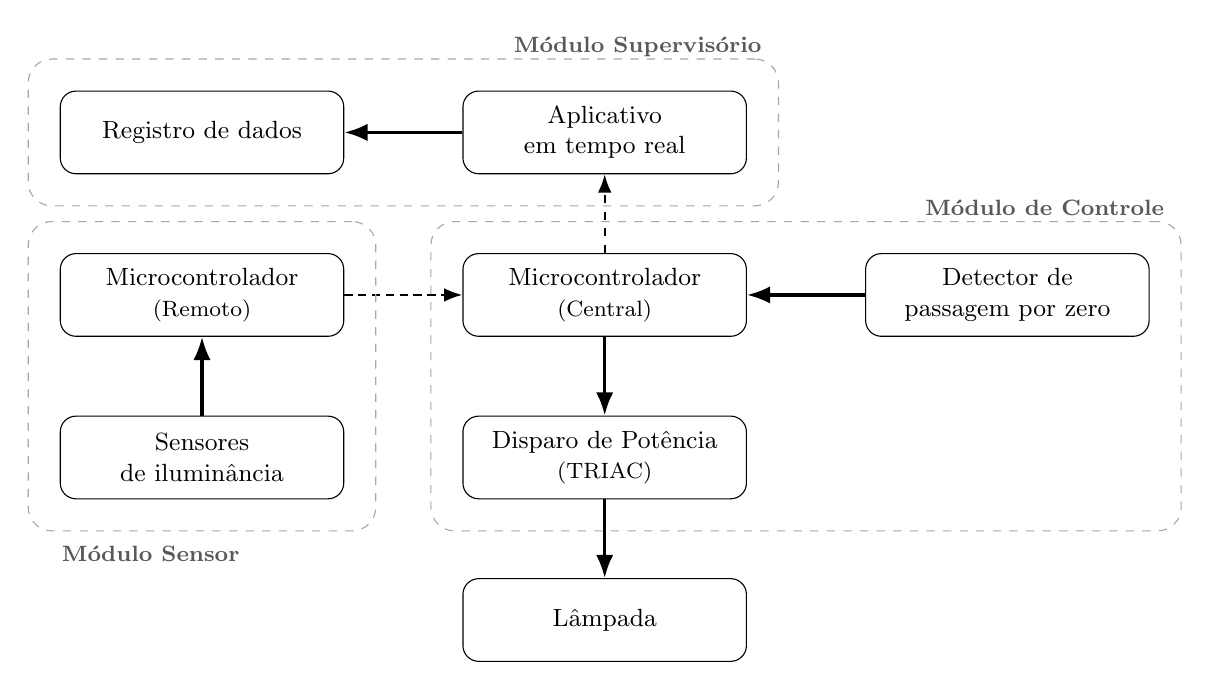
\begin{tikzpicture}[
  font=\small,
  node distance=10mm and 15mm,
  block/.style={draw, rounded corners=2mm, align=center, minimum width=3.6cm, minimum height=1.05cm},
  main/.style={-Latex, very thick},
  comm/.style={-Latex, thick, densely dashed},
  aux/.style={-Latex, dashed, thick},
  group/.style={draw, rounded corners=3mm, dashed, gray!70, inner sep=4mm}
]

% --- Linha superior ---
\node[block] (mcur) {Microcontrolador \\ \footnotesize(Remoto)};
\node[block, right=of mcur] (ctrl) {Microcontrolador \\ \footnotesize(Central)};
\node[block, right=of ctrl] (zc) {Detector de \\ passagem por zero};

% --- Linha inferior ---
\node[block, below=of mcur] (sens) {Sensores\\ de iluminância};
\node[block, below=of ctrl] (drv) {Disparo de Potência\\ \footnotesize(TRIAC)};
\node[block, below=of drv] (load) {Lâmpada};

% --- Supervisório e registro ---
\node[block, above=of ctrl] (sup) {Aplicativo\\ em tempo real};
\node[block, above=of mcur] (log) {Registro de dados};

% --- Conexões principais ---
\draw[main] (sens) -- (mcur);
\draw[comm] (mcur) -- (ctrl);
\draw[main] (ctrl) -- (drv);
\draw[main] (drv) -- (load);
\draw[main] (zc) -- (ctrl);

% --- Supervisório e logging ---
\draw[aux] (ctrl) -- (sup);
\draw[main] (sup) -- (log);

% --- Contornos (grupos) ---
\node[group, fit=(mcur)(sens)] (gSens) {};
\node[group, fit=(ctrl)(zc)(drv)] (gCtrl) {};
\node[group, fit=(log)(sup)] (gSup) {};

% --- Rótulos dos grupos ---
\node[font=\bfseries\footnotesize, gray!70!black, anchor=south east]
  at ([xshift=6mm,yshift=-5mm]gSens.south) {Módulo Sensor};
\node[font=\bfseries\footnotesize, gray!70!black, anchor=south east]
  at ([xshift=-1mm,yshift=-0.5mm]gCtrl.north east) {Módulo de Controle};
\node[font=\bfseries\footnotesize, gray!70!black, anchor=south east]
  at ([xshift=-1mm,yshift=-1mm]gSup.north east) {Módulo Supervisório};


\end{tikzpicture}
\caption{Diagrama de blocos do sistema: sensoriamento, controle e supervisão.}
\label{fig:diag_blocos_sistema}
\end{figure}

\section{Projeto do Módulo de Controle}

O Módulo de Controle é o elemento central do sistema, ele é o responsável por receber as medições, processar os dados, executar o algorítmo de controle, comandar o acionamento da carga e gerenciar a comunicação do sistema.

Os pontos centrais para o projeto foram:
\begin{itemize}
    \item Método de controle de potência;
    \item Isolamento entre os estágios lógico e de potência;
    \item Execução em tempo real;
    \item Confiabilidade na comunicação;
    \item Eficiência energética e robustez.
\end{itemize}

Com base nesses pontos o circuito do módulo de controle foi desenvolvido no software \textit{KiCad} como mostra a Figura \ref{fig:proj_contr}

\subsection{Hardware}

\subsubsection{Microcontrolador}

O microcontrolador é o núcleo do módulo de controle, a escolha do dispositivo adequado influencia diretamente o desempenho, a estabilidade e a eficiência do sistema embarcado. 
A Tabela~\ref{tab:microcontroladores} apresenta um comparativo entre os principais modelos considerados para este projeto, destacando os parâmetros técnicos mais relevantes para a aplicação.


\begin{table}[htb]
  \centering
  \caption{Comparativo entre microcontroladores candidatos ao módulo de controle.}
  \begin{tabular}{m{3.5cm}m{2.4cm}m{2.2cm}m{2.6cm}m{3.8cm}}
    \Linha % linha grossa
    {\bf Modelo} & {\bf Arquitetura} & {\bf Frequência} & {\bf Comunicação} & {\bf Observações} \\
    \Linha % linha grossa
    Arduino Uno & 8 bits & 16 MHz & UART, I\textsuperscript{2}C, SPI & Baixo custo e simplicidade, porém desempenho limitado para controle em tempo real. \\
    \hline
    ESP8266 (NodeMCU-V3) & 32 bits & 80 MHz & UART, SPI, I\textsuperscript{2}C, Wi-Fi & Boa conectividade Wi-Fi, mas poucos recursos de E/S e menor capacidade de processamento. \\
    \hline
    ESP32-S (NodeMCU-32S) & 32 bits Dual-Core & 240 MHz & UART, SPI, I\textsuperscript{2}C, Wi-Fi, BLE & Alto desempenho e conectividade dupla (Wi-Fi e BLE), ideal para controle em tempo real e comunicação com sensores e supervisório. \\
    \Linha % linha grossa
  \end{tabular}    
  \FonteTab{Próprio autor, com base em \cite{Espressif, Arduino, EspressifESP8266}.}
  \label{tab:microcontroladores}
\end{table}

Com base nesses fatores, o microcontrolador \textit{ESP32-S (NodeMCU-32S)} foi selecionado para o módulo de controle. 
A escolha se deve ao seu processador \textit{dual-core} de até 240 MHz, que permite a execução simultânea do algoritmo fuzzy e das rotinas de comunicação, além do suporte nativo a \textit{Wi-Fi} e \textit{Bluetooth} de Baixa Energia (\gls{BLE}), que viabiliza a integração com os módulos sensores e o sistema supervisório. 
Essas características garantem baixo tempo de resposta, estabilidade de comunicação e alta eficiência energética, fatores essenciais para a operação do sistema em tempo real.

\subsubsection{Alimentação}

O circuito de alimentação deve fornecer energia estável para todos os componentes do módulo de controle, para essa função foi escolhido o módulo conversor HLK-5M05, que converte a tensão de entrada de 127/220 V CA para uma saída de 5 V CC regulada, com corrente máxima de 1 A.

Além do módulo conversor, foi implementada uma etapa de filtragem utilizando dois capacitores em paralelo: um eletrolítico de 100 µF e um cerâmico de 100 nF. Essa associação é recomendada por ampliar a faixa de atenuação de ruídos. \cite{TexasInstr630}

\subsubsection{Detector de Pasagem por Zero}

O controle de potência empregado neste projeto baseia-se no método de corte de fase
para que o controle seja preciso e estável, é indispensável identificar o momento exato em que a tensão alternada cruza o valor zero. Esse sincronismo garante que o disparo do TRIAC ocorra de forma coerente com a fase da rede elétrica, evitando oscilações de brilho, ruídos eletromagnéticos e distorções harmônicas. Com isso torna-se necessário o uso de um circuito detector de passagem por zero.

O detector de passagem por zero sincroniza o controle ao detectar quando a tensão muda de polaridade \cite{Vieira2024}. O circuito utiliza uma ponte retificadora para gerar uma forma de onda pulsante e um optoacoplador para garantir o isolamento elétrico entre os estágios de potência e controle, a cada cruzamento por zero, o pulso gerado é identificado pelo microcontrolador.

A ponte retificadora 2W10 foi selecionada por suportar correntes e tensões reversas superiores às condições de operação do circuito de detecção, além de apresentar encapsulamento compacto e fácil integração na placa de circuito impresso.

O optoacoplador 4N25 foi adotado por sua ampla disponibilidade, baixo custo e características ideais para a função de isolamento entre os estágios de potência e controle. O dispositivo oferece alta imunidade a ruídos e tempo de comutação compatível com a frequência da rede elétrica, permitindo detectar com precisão o instante de passagem por zero.

\subsubsection{Circuito de Disparo de Potência}

O circuito de disparo de potência é responsável por controlar o momento de condução da corrente alternada que alimenta a lâmpada, permitindo o ajuste de sua intensidade luminosa. Ele utiliza o optoacoplador MOC3021M, que garante isolamento entre o microcontrolador e a rede elétrica, e o TRIAC BT136, responsável pela comutação da carga. Como o MOC3021M é um modelo sem detecção de cruzamento por zero, o disparo pode ocorrer em qualquer ponto do semiciclo da rede, possibilitando o controle por corte de fase realizado pelo algoritmo fuzzy do sistema.

O sinal de disparo gerado pelo microcontrolador aciona o LED interno do MOC3021M por meio de um resistor limitador, conduzindo o pulso ao gate do BT136, que passa a conduzir até o final do semiciclo. Dessa forma, ao variar o atraso do pulso de disparo, é possível ajustar a potência entregue à lâmpada.

\subsection{Firmware}

O módulo de controle possui um firmware desenvolvido para o microcontrolador ESP32-S, responsável por gerenciar a comunicação entre os módulos, executar o ciclo de controle fuzzy que regula a luminosidade do ambiente e verificar possíveis erros alertando o usuário.

\subsubsection{Arquitetura Geral}

A arquitetura geral do firmware é baseada em uma máquina de estados que gerencia o funcionamento do sistema em diferentes modos operacionais sendo eles: Esperando sensores; Controle ativo; Estabilizando; Sensores em \textit{standby}; Retomada pós-\textit{standby}. As transições entre os estados são acompanhadas por processos de registro, atualização de contadores e configuração de temporizadores, garantindo que o sistema funcione de forma ordenada e previsível.

\subsubsection{Inicialização do firmware}

Durante a inicialização o controlador configura os principais recursos de hardware e software necessários para o funcionamento do sistema, essa fase inclui:
\begin{itemize}
    \item \textbf{Carregamento de parâmetros armazenados,} como \textit{setpoint} e modo de operação, a partir da memória não volátil;
    \item \textbf{Configuração dos pinos e temporizadores,} incluindo a detecção de passagem por zero;
    \item \textbf{Inicialização do controle fuzzy,} com a definição dos conjuntos de pertinência e da base de regras;
    \item \textbf{Estabelecimento da comunicação de rede,} permitindo a troca de informações com o Módulo Supervisório;
    \item \textbf{Entrada no estado de espera dos sensores,} mantendo a lâmpada desligada até que todas as condições de operação estejam seguras.
\end{itemize}

Essas etapas garantem que o sistema funcione apenas com a configuração completa de todos os subsistemas.

\subsubsection{Ciclo principal}

O ciclo principal do firmware coordena três tarefas centrais:
\begin{itemize}
    \item \textbf{Aquisição e validação de dados:} as leituras provenientes dos sensores são atualizadas e filtradas, mantendo a coerência das informações e detectando automáticamente falhas de  comunicação dos sensores;
    \item \textbf{Execução do controle fuzzy:} o controlador compara a iluminância medida com o \textit{setpoint} e aplica a lógica fuzzy gerando um novo percentual de ajuste da lâmpada;
    \item \textbf{Gestão de estados e \textit{standby}:} temporizadores determinam os intervalos de estabilização e de \textit{standby}. Durante o modo \textit{standby} os sensores entram em baixa atividade e a potência da lâmpada é mantida até o reinício do ciclo de controle.
\end{itemize}

\subsubsection{Lógica fuzzy}

O controle do sistema é realizado com base numa lógica fuzzy projetada para o ajuste de potência da lâmpada conforme a variação da iluminância ambiente. Três variáveis linguísticas compõem a base de regras:
\begin{itemize}
    \item \textbf{Erro,} subtração entre o \textit{setpoint} e a iluminância medida, organizado em cinco conjuntos: muito abaixo, abaixo, pequeno, acima e muito acima;
    \item \textbf{Variação do Erro,} diferença entre o erro atual e o erro anterior, ordenada em três conjuntos: diminuição rápida, estável e aumento rápido;
    \item \textbf{Ajuste de Potência,} variável de saída que determina o percentual da potência que deve ser ajustada, compreendida em 5 conjuntos: diminuir muito, diminuir, manter, aumentar e aumentar muito.
\end{itemize}

A base de regras foi desenvolvida para garantir respostas rápidas quando o erro está elevado ao mesmo tempo em que corrige suavemente quando o erro está próximo a zero. O processo fuzzyfica as entradas, aplica inferência do tipo Mamdani e defuzzyfica pelo método do centroide.

\subsubsection{Acionamento do TRIAC}

O acionamento da carga é ralizado por meio de um circuito de disparo de TRIAC, sincronizado a rede elétrica. O firmware converte o percentual de potência calculado pelo controle fuzzy em um tempo de atraso do disparo, controlando assim a fração de condução desejada em cada semiciclo da tensão alternada.

Tabelas e rotinas de interpolação garantem a correspodência entre o valor de potência e o tempo de disparo. Interrupções independentes controlam o instante do disparo e o desligamento do pulso, mantendo o sincronismo e garantindo que outras tarefas do microcontrolador não vão atrapalhar o acionamento do TRIAC.

\subsubsection{Comunicação e validação}

O controlador comunica-se com os sensores por meio de \gls{BLE} e com o sistema externo por meio de \textit{Wi-Fi}, garantindo a troca contínua de dados de iluminância e parâmetros de operação. As mensagens recebidas passam por verificação de integridade e consistência, prevenindo falhas causadas por leituras incorretas ou atrasadas.
O firmware também monitora o estado dos sensores e da potência aplicada, adotando modo seguro em caso de perda de comunicação, saturação ou ausência de dados. As últimas configurações válidas são gravadas na memória não volátil, permitindo a retomada estável do controle após reinicializações.

\section{Projeto do Módulo Sensor}

O Módulo Sensor é responsável por medir a iluminância do ambiente e transmitir esses dados para o Módulo de Controle. Ele atua de forma independente e distribuída, permitindo a instalação de múltiplos sensores em diferentes locais do ambiente.

Os pontos centrais para o projeto foram:
\begin{itemize}
    \item Precisão nas medições de iluminância;
    \item Baixo consumo energético e operação autônoma;
    \item Comunicação confiável e sem fio;
    \item Compactação do circuito.
\end{itemize}

Baseado nesses requisitos, o circuito do módulo sensor foi desenvolvido no software \textit{KiCad} como mostra a Figura \ref{fig:proj_sens}.

\subsection{Hardware}

\subsubsection{Microcontrolador}

O microcontrolador é o núcleo do módulo sensor, responsável por coletar os dados do sensor de iluminância e transmiti-los ao módulo de controle. A Tabela~\ref{tab:microcontroladores_sensores} apresenta um comparativo entre os principais modelos considerados para este projeto, destacando os parâmetros técnicos mais relevantes para a aplicação.

\begin{table}[htb]
  \centering
  \caption{Comparativo entre microcontroladores candidatos ao módulo de sensores.}
  \begin{tabular}{m{3.5cm}m{2.4cm}m{2.2cm}m{2.6cm}m{3.8cm}}
    \Linha % linha grossa
    {\bf Modelo} & {\bf Arquitetura} & {\bf Frequência} & {\bf Comunicação} & {\bf Observações} \\
    \Linha % linha grossa
    ESP8266 (NodeMCU-V3) & 32 bits & 80 MHz & UART, SPI, I\textsuperscript{2}C, Wi-Fi & Boa conectividade Wi-Fi e baixo custo, porém ausência de BLE nativo, o que limita a comunicação direta com o controlador. \\
    \hline
    ESP32-S (NodeMCU-32S) & 32 bits Dual-Core & 240 MHz & UART, SPI, I\textsuperscript{2}C, Wi-Fi, BLE & Alto desempenho e conectividade dupla (Wi-Fi e BLE), porém com maior consumo e dimensões que dificultam o uso em módulos compactos alimentados por bateria. \\
    \hline
    ESP32-C3 (Super-Mini) & 32 bits RISC-V & 160 MHz & UART, SPI, I\textsuperscript{2}C, Wi-Fi, BLE & Combina BLE nativo, baixo consumo e formato reduzido, ideal para módulos distribuídos de medição. \\
    \Linha % linha grossa
  \end{tabular}
  \FonteTab{Próprio autor, com base em \cite{Espressif, EspressifESP8266, EspressifC3}.}
  \label{tab:microcontroladores_sensores}
\end{table}

Com base nesses fatores, o microcontrolador \textit{ESP32-C3 (Super-Mini)} foi selecionado para o módulo sensor. A escolha se deve ao seu tamanho compacto com desempenho suficiente para a aquisição e transmissão dos dados de iluminância, além do suporte nativo a \gls{BLE}, que viabiliza a comunicação eficiente com o Módulo de Controle.

\subsubsection{Sensor de Iluminância}

O sensor de iluminância escolhido para o módulo sensor foi o \textit{BH1750}, um sensor digital de alta precisão que utiliza comunicação I\textsuperscript{2}C para transmitir os dados de iluminância ao microcontrolador. O \textit{BH1750} oferece uma faixa de medição de 1 a 65535 lux, com resolução de 1 lux, apresentando erro típico de ±20\%. Além disso, seu tempo de conversão é ajustável entre 120 ms e 180 ms, o que oferece uma boa relação entre velocidade de resposta e estabilidade de leitura. O consumo típico é de 0,12 mA durante a medição e 0,01 µA em modo de espera, características que o tornam adequado para sistemas alimentados por bateria.

\subsubsection{Alimentação}

O módulo de sensores é alimentado por um conjunto de duas baterias 18650 de 2200 mAh ligadas em série, fornecendo tensão nominal de 7,4 VCC, suficiente para operação autônoma e sem fio. Essa tensão é reduzida para 3,3 VCC pelo conversor DD4012SA, um regulador DC-DC step-down de alta eficiência ($\simeq 90\%$), com corrente de saída de até 1,2 A, garantindo alimentação estável para o ESP32-C3 e o BH1750 com baixo aquecimento.

\subsection{Firmware}

O firmware foi desenvolvido para realizar a leitura periódica da iluminância, transmitir os dados ao controlador via BLE e gerenciar o consumo energético. A estrutura modular do código permite a replicação de vários sensores com configuração individual, sem necessidade de alterações estruturais no programa.

\subsubsection{Inicialização e comunicação}
Durante a inicialização, o microcontrolador configura o barramento de comunicação e ativa o sensor de iluminância em modo de medição de alta precisão. Após a verificação de funcionamento, estabelece-se a comunicação \gls{BLE}, por meio da qual o módulo é identificado individualmente dentro da rede de sensores e passa a transmitir as leituras de iluminância.

\subsubsection{Transmissão e gerenciamento de dados}
O firmware implementa um serviço de comunicação padronizado, capaz de enviar medições e receber comandos do controlador principal. Essa troca contínua garante a sincronização dos dados e permite, por exemplo, o acionamento remoto do modo de economia de energia ou a atualização de parâmetros de medição. Caso ocorra perda de conexão, o módulo reinicia automaticamente o processo de publicidade \gls{BLE} até que o vínculo seja restabelecido, assegurando continuidade na transmissão das informações.

\subsubsection{Economia de energia}
A estratégia de economia de energia combina o modo de espera do sensor com o modo de sono profundo do microcontrolador, definindo um ciclo de repouso de aproximadamente cinco minutos entre as leituras. Durante esse intervalo, apenas os circuitos essenciais permanecem ativos, reduzindo significativamente o consumo médio. Essa abordagem garante autonomia prolongada das baterias e operação estável em longo prazo, mantendo a confiabilidade das medições em campo.


\section{Projeto do Módulo Supervisório}



%%%%%%%%%%%%%%%%%%%%%%%%%%%%%%%

\chapter{Validação do Sistema}

%%%%%%%%%%%%%%%%%%%%%%%%%%%%%%%

\chapter{Discussão dos Resultados}

%%%%%%%%%%%%%%%%%%%%%%%%%%%%%%%

\chapter{Análise dos Resultados}

%%%%%%%%%%%%%%%%%%%%%%%%%%%%%%%
% \include{Outro_Capitulo}
% \include{Mais_um_Capitulo}
% \include{Mais_outro_Capitulo}
% \include{}
% \include{}
%
%%% não altere este documento 
%%%%%%%%%%%%%%%%%%%%%%%%%%%%
% Este documento pertence à classe cls-PFC-COEEL.cls
% NÃO ALTERE NADA AQUI
%%%%%%%%%%%%%%%%%%%%%%%%%%%%
%
% Apenas para PFC
%
\ifpfc % se é PFC
   \include{./PFC_Especificos/j_Consideracoes_Finais}
   \include{./PFC_Especificos/k_Sugestoes_Trab_Futuros}
\fi 
%
%%%%%%%%%%%%%%%%%%%%%%%%%%%%%%
%%%%%%%%%%%%%%%%%%%%%%%%%%%%
%%%% CRONOGRAMA
%
% Apenas para Pré-Projeto
%
\ifpreprojeto % se é Pré-Projeto
   %%%%%%%%%%%%%%%%%%%%%%%%%%%%%%%%%%%%%%%%
%
% o CRONOGRAMA é obrigatório 
% APENAS PARA PRÉ-PROJETO de PFC
%
%%%%%%%%%%%%%%%%%%%%%%%%%%%%%%%%%%%%%%%%

\chapter{CRONOGRAMA}

O cronograma deste trabalho está organizado em fases que abrangem desde a pesquisa teórica até a implementação prática do projeto. A primeira etapa consiste no levantamento bibliográfico e estudo dos fundamentos teóricos necessários para o desenvolvimento do sistema. Em seguida, serão realizados o projeto e a simulação do circuito, seguidos pela montagem e testes do protótipo. A fase final inclui a análise dos resultados, a redação do trabalho e a preparação para a apresentação. Cada etapa foi planejada de forma a garantir o cumprimento dos prazos e a qualidade do trabalho entregue, conforme tabela~\ref{tab:Cronograma}.

\begin{table}[htb]
  \centering
  \caption{Cronograma de Execução do Projeto Final de Curso}
  \begin{tabular}{m{6cm}cccccc} % l=Left(textos); r=Right(números); o comando m{6cm} fixa a primeira coluna em 6cm, faz quebra de linha e centraliza as demais colunas na vertical
    \Linha % linha grossa
    {\bf CRONOGRAMA PFC-2025} & {\bf Jul} & {\bf Ago}  & {\bf Set} & {\bf Out} & {\bf Nov} & {\bf Dez}  \\
    \Linha % linha grossa      
    Levantamento bibliográfico & X &   &   &   &   &     \\
    \hline % linha fina
    Alinhamento da proposta    & X &   &   &   &   &     \\
    \hline % linha fina
    Projeto                    &   & X &   &   &   &     \\
    \hline % linha fina
    Montagem e experimentos    &   & X & X &   &   &     \\
    \hline % linha fina
    Levantamento de dados,   
    criação de tabelas e 
    gráficos                   &   &   &  X &   &   &    \\
    \hline
    Escrita da monografia      &   &   &  X &  X  &   &  \\
    \hline % linha fina
    Revisão da monografia      &   &   &  X &  X  &   &  \\
    \hline  
    Defesa perante Banca       &   &   &    &     &  X &    \\
    \Linha % linha grossa
  \end{tabular}    
  \FonteTab{Próprio Autor}
  \label{tab:Cronograma}
\end{table}

\fi 
%
%%%%%%%%%%%%%%%%%%%%%%%%%%%%
%%%%%%%%%%%%%%%%%%%%%%%%%%%%
%%%% REFERÊNCIAS
%
\ifpdf\phantomsection\fi
\addcontentsline{toc}{chapter}{REFERÊNCIAS}
\renewcommand{\bibname}{REFERÊNCIAS}
\bibliography{BIB_pfc} % nome do seu arquivo bib
\label{cap:RefBib}
%
%%%%%%%%%%%%%%%%%%%%%%%%%%%%
%%%%%%%%%% AQUI VÃO SEUS APÊNDICES %%%%%%%%%%%%
%%%%%%%%%%%%%%%%%%%%%%%%%%%%
% APÊNDICE são textos criados pelo próprio autor para complementar sua argumentação (ABNT NBR14724)
%
% Apenas para PFC
%
\ifpfc % se é PFC
    \chapter{APÊNDICES}

\begin{figure}[htb]
   \centering
   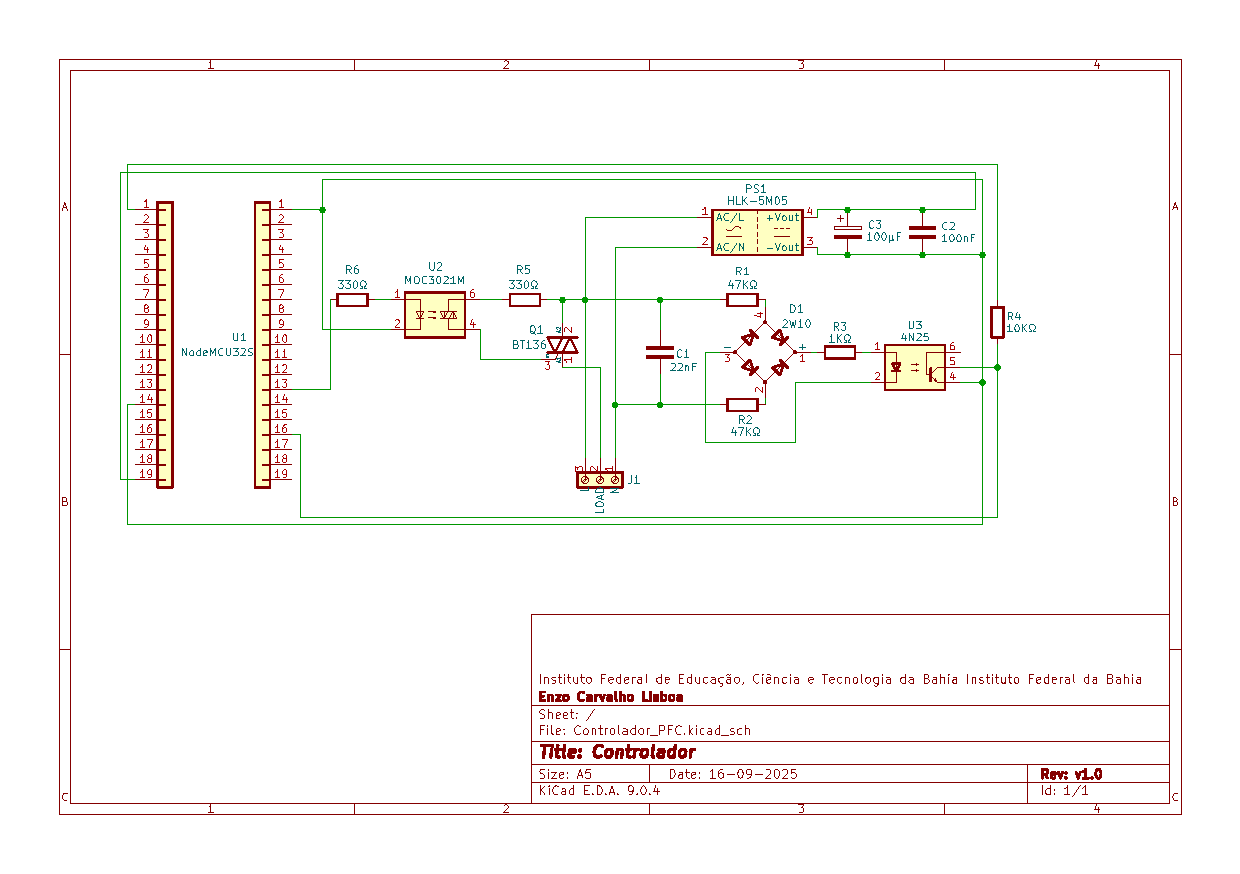
\includegraphics[angle=90, width=15.4cm]{./arquivos/Controlador.pdf} % PDF, PNG, JPG
   \caption{Projeto do circuito do controlador}
   \label{fig:proj_contr}
\end{figure}

\begin{figure}[htb]
   \centering
   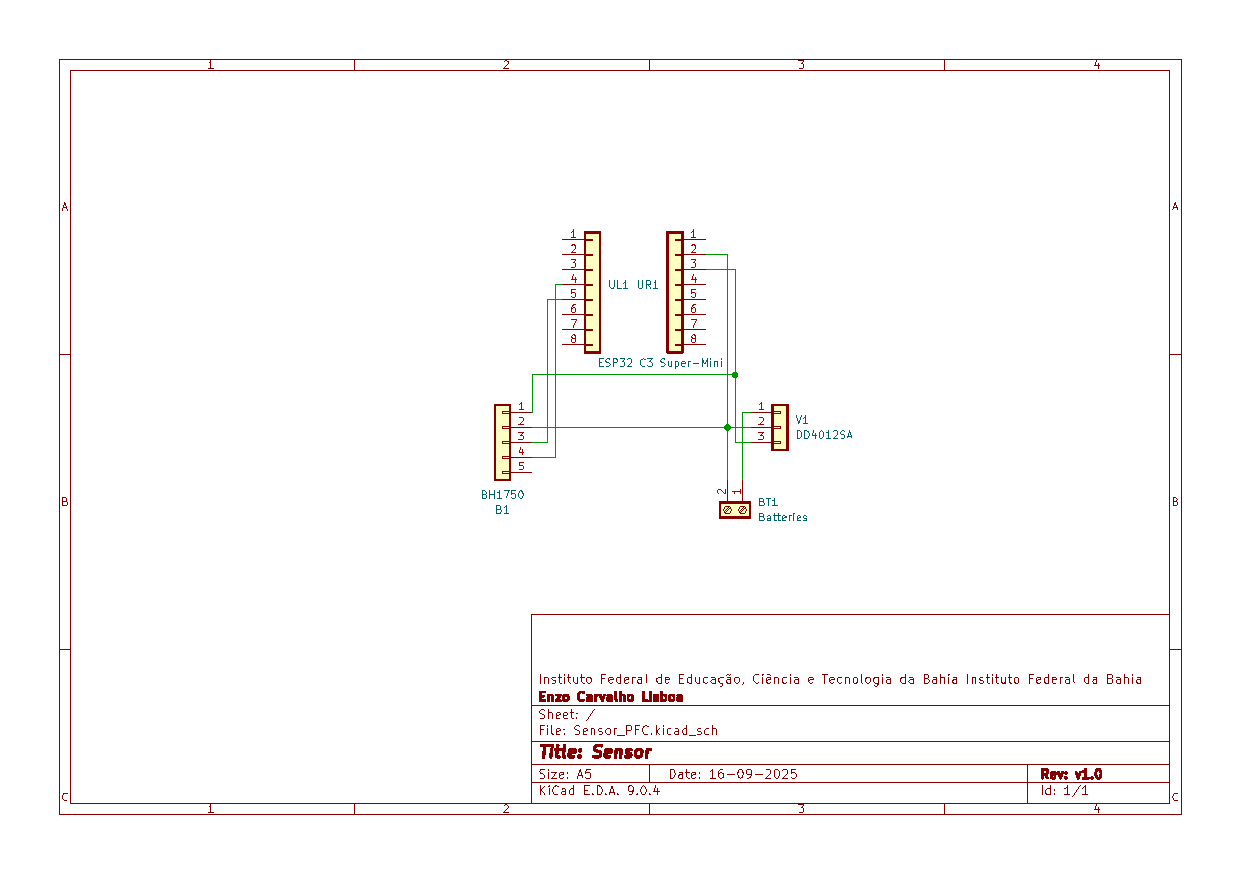
\includegraphics[angle=90, width=15.4cm]{./arquivos/Sensor.pdf} % PDF, PNG, JPG
   \caption{Projeto do circuito do sensor}
   \label{fig:proj_sens}
\end{figure}

\fi 
%
%%%%%%%%%%%%%%%%%%%%%%%%%%%%
%%%%%%%%%% AQUI VÃO SEUS ANEXOS  %%%%%%%%%%%%%%
%%%%%%%%%%%%%%%%%%%%%%%%%%%%
% ANEXOS são documentos criados por terceiros, e usados pelo autor (ABNT NBR14724)
%
% Apenas para PFC
%
\ifpfc % se é PFC
    %%%%%%%%%%%%
\chapter*{ANEXOS}
\addcontentsline{toc}{chapter}{ANEXOS}

\fi 
%
%
%%%%%%%%%%%%%%%%%%%%%%%%%%%%
%%%%%%%%%%%%%%%%%%%%%%%%%%%%
%%%% ÍNDICE REMISSIVO
%
% Apenas para PFC
%
\ifpfc % se é PFC
    \clearpage\pagebreak\newpage
    \ifpdf\phantomsection\fi
    \renewcommand{\indexname}{ÍNDICE REMISSIVO}
    \addcontentsline{toc}{chapter}{\indexname}
    \printindex  % índice remissivo
\fi 
%
%%%%%%%%%%%%%%%%%%%%%%%%%%%%%%



%%%%%%%%%%%%%%%%%%%%%%%%%%%%
%
\end{document}
%
%%%%%%%%%%%%%%%%%%%%%%%%%%%%
%%%%%%%%%%%  FIM  %%%%%%%%%%%%%%%%%%%%%%%%%%%%
%%%%%%%%%%%%%%%%%%%%%%%%%%%%